% Appunti del corso Fondamenti dell'Informatica a.a. 2017/2018 
% Autore: Alessandro Righi <alessandro.righi@outlook.it>
% Questo documento è rilasciato con licenza GPLv3
% Sono quindi ben accette correzioni di errori, aggiunte, migliorie, ecc. 
% Chi volesse suggerirmi cambiamenti mi contatti pure all'indirizzo mail sopra indicato. 

\documentclass[a4paper,titlepage]{article}
\usepackage[italian]{babel}
\usepackage[T1]{fontenc}
\usepackage[utf8x]{inputenc}
\usepackage{amsmath}
\usepackage{amsfonts}
\usepackage{amsthm}
\usepackage{graphicx}
\usepackage{frontespizio}
\usepackage{tikz}
\usepackage[a4paper]{geometry}
\usepackage{mathtools}
\usepackage{pgfplots}
\usepackage{enumerate}
\usepackage{amssymb}
\usepackage{verbatim}
\usepackage[siunitx]{circuitikz}
\usepackage{calrsfs}
\usepackage{algpseudocode}

\usetikzlibrary{shapes, arrows, positioning, automata}

\newtheorem{theorem}{Teorema}[section]
\newtheorem{lemma}{Lemma}[section]
\newtheorem{definition}{Definizione}[section]
\newtheorem{corollario}{Corollario}[section]
\theoremstyle{definition}
\newtheorem*{example}{Esempio}

\newcommand{\CFG}{\langle V,T,P,S\rangle}
\newcommand{\DFA}{\langle Q,\Sigma,\delta,q_0,F\rangle}
\newcommand{\N}{\mathbb{N}}

\begin{document}
	
\begin{frontespizio}
	\Preambolo{\usepackage{datetime}}
	\Istituzione{Università degli Studi di Verona}
	\Divisione{Dipartimento di Informatica}
	\Scuola{Ultima modifica: \today }
	\Titolo{Fondamenti dell'Informatica}
	\Sottotitolo{Appunti}
	\Candidato{Alessandro Righi}
	\NCandidato{Autore}
	\Annoaccademico{2017/2018}
\end{frontespizio}

\tableofcontents
\newpage

\section{Introduzione}
Questi appunti di Fondamenti dell'Informatica sono stati scritti relativamente al corso tenuto dal mitico prof. Roberto Giacobazzi nell'anno accademico 2017/2018. Ho cercato di fare un riassunto non troppo breve degli argomenti del corso inserendo le dimostrazioni più richieste e importanti. 

Gli appunti sono stati scritti più che altro per l'esame orale quindi includono essenzialmente solo la parte teorica e non gli esercizi dell'esame. Ho inserito i teoremi principali e le dimostrazioni dei più importanti, spesso lasciando però stare il formalismo preciso ma piuttosto descrivendo l'idea che ci sta dietro. 

Questa dispensa la ho scritta abbastanza di fretta e per aiutarmi nello studio, quindi è molto certo che all'interno vi siano errori, parti poco chiare, parti da migliorare,  approfondire, aggiungere, cestinare: ai posteri lascio questo compito, ogni modifica è ben accetta, il codice sorgente \LaTeX è disponibile su GitHub, sentitevi quindi liberi di fare pull request o chiedere a chi gestisce il repository ossia Davide Bianchi l'accesso. Per chi volesse contattarmi via email mi scriva ad alessandro.righi@outlook.it.

\section{Concetti basilari}
Vediamo alcuni concetti base da introdurre prima del corso. Molte cose dovrebbero essere state già viste in logica comunque. 

\subsection{Sistemi formali}
Un \textit{sistema formale} $S$ e un sistema di formule e regole per combinare formule, descritto mediante un insieme finito (numerabile) di simboli $S$, e tale che per ogni regola $R\subseteq S^k$ per qualche $k\in\N$ sia possibile stabilire in modo decidibile se una formula $f$ è conseguenza di $f_1,\dots,f_{k-1},f$ secondo $R$, ossia se $\langle f_1,\dots,f_{k-1},f\rangle\in R$ 

\begin{definition}[relazione binaria]
	Una relazione binaria $R$ è un sottoinsieme del prodotto cartesiano di due insiemi $A$ e $B$: $R \subseteq A \times B$
\end{definition}

\begin{definition}[chiusura transitiva]
	La chiusura transitiva di una relazione  $R \subseteq S\times S $ è il più piccolo insieme $ R^{* }$ tale che $ R \subseteq R^{*} \wedge (\langle a, b \rangle \in R^{*} \wedge \langle b, c \rangle \in R^{*} \implies \langle a, c \rangle \in R^{*}) $
\end{definition}

Definiamo la chiusura transitiva per induzione come $R^* = \bigcup_{i \in\N} R^i$ dove:
\[
	\begin{cases}
		R^1 = R \\
		R^{n+1} = {\langle a, c \rangle : \langle a, b \rangle \in R^i \wedge \rangle b, c \langle in R}
	\end{cases}
\]

\begin{definition}[ordine parziale]
	Una relazione binaria $R\subseteq S\times S$ è un ordine parziale se è un riflessiva, transitiva e antisimmetrica. 
\end{definition}

\begin{definition}[relazione ben fondata]
	Una relazione binaria $R\subseteq S\times S$ è ben fondata se per ogni $Y\subseteq S, Y \neq\varnothing$ esiste $z\in Y$ tale che $\langle y, z \rangle\notin R$ per ogni $y\in Y\setminus \{z\}$. Se $R$ è ben fondata, $S$ è detto insieme ben fondato.
\end{definition}

Se $R\subseteq S\times S$ è una relazione di ordine parziale, essa è ben fondata se ogni $Y\subseteq S, Y\neq\varnothing$ ha un elemento minimale. Un insieme è ben fondato se ha quindi un elemento minimale. 

\subsection{Chiusura di Kleene}
Sia $\Sigma$ un alfabeto e $L,L_1,L_2$ insiemi di stringhe di $\Sigma^*$. La concatenazione di $L_1$ e $L_2$ è l'insieme: 
\[
	L_1 L_2 = \{xy\in\Sigma^*:x\in L_1, y\in L_2\}
\]
Definiamo: 
\[
	\begin{cases} 
		L^0=\{\varepsilon\}\\
		L^{i+1}=LL^i
	\end{cases}
\]
La \textit{chiusura di Kleene di L}, denotata come $L^*$ è l'insieme: 
\[
	L^*=\bigcup_{i\geq0}L^i
\]

\subsection{Principio di induzione}
Il principio di induzione è un punto fondamentale, che verrà usato praticamente sempre quando ci sarà da dimostrare un teorema, quindi è bene capirne perfettamente il suo funzionamento. 

\begin{theorem}[induzione ben fondata]
	Sui $(S, \prec)$ un insieme ben fondato e sia $\phi(x)$ una proprietà su $S$. Allora se $\forall x\in S.\forall y,y\prec x.\phi(y)\Rightarrow\phi(x)$ allora $\forall x\in S.\phi(x)$
\end{theorem}

Intuitivamente, se devo dimostrare che una proprietà vale su tutto un insieme $S$, mi basta dimostrare che la proprietà vale per gli elementi minimali di $S$ (caso base), e poi dimostrare che se la proprietà vale per $n$ allora vale anche per $n+1$ (caso induttivo). In questo modo posso asserire che la proprietà vale su tutto $S$ senza averla verificata per ogni singolo elemento (che, nel caso di insiemi infiniti sarebbe impossibile)

\part{Linguaggi formali}
\section{Automi}
\subsection{Automi a stati finiti deterministici}
Un \textit{automa a stati finiti deterministico} (\textbf{DFA}) è una macchina estremamente semplice: essa non ha a disposizione una memoria, ma ricorda solo lo stato corrente in cui si trova. La macchina legge da un nastro di input dei simboli appartenenti ad un alfabeto, ed in base al simbolo letto e lo stato corrente in cui esegue una transizione in un nuovo stato (o rimane nello stesso stato con un autotransizione). 

Quando tutta la stringa di input è stata letta, ossia non vi sono più simboli presenti sul nastro di input, l'automa si può trovare in uno stato finale, o di accettazione, in tal caso si dirà che l'automa ha riconosciuto la stringa ed essa appartiene al linguaggio della macchina, o in uno stato non finale e quindi la stringa non apparterrà al linguaggio dell'automa. 

Formalmente possiamo descrivere un DFA con una quintupla $\DFA$, dove:
\begin{itemize}
	\item $Q$ è l'insieme degli stati dell'automa 
	\item $\Sigma$ è l'alfabeto di input 
	\item $\delta: Q \times \Sigma \to Q$ la funzione di cambiamento di stato 
	\item $q_0$ lo stato iniziale 
	\item $F \subseteq Q$ l'insieme degli stati finali
\end{itemize}


Dalla funzione $\delta$ definiamo ricorsivamente la funzione $\hat\delta: Q\times\Sigma^{*} \to Q$ che ci tornerà utile in seguito:
\[
	\begin{cases}
		\hat\delta(q,\varepsilon)=q\\
		\hat\delta(q,\sigma a)=\delta(\hat{\delta}(q, \sigma), a)  
	\end{cases}
\]

Possiamo rappresentare l'automa come un grafo in cui i nodi sono gli stati e gli archi le transizioni:
\begin{center}
	\begin{tikzpicture}[shorten >=1pt,node distance=2cm,on grid]
		\node[state,initial] (q0) {$q_0$};
		\node[state,accepting] (q1) [above right=of q0] {$q_2$};
		\node[state] (q2) [below right=of q0] {$q_1$};
		\path[->] 
			(q2) edge [loop above] node [above] {a,b} ()
			(q0) edge [bend right] node [above] {a} (q1)
			(q0) edge node [above] {b} (q2)
			(q1) edge [loop above] node [above] {a} ()
			(q1) edge [bend right] node [above] {b} (q0);
	\end{tikzpicture}
\end{center}

La tabella di transizione per il precedente automa è:
\begin{center}
	\begin{tabular}{l | l | l}
					& $a$ 	& $b$	\\ \hline
		$q_0$  & $q_2$	& $q_1$	\\
		$q_1$   & $q_1$ & $q_1$	\\
		$q_2$  & $q_2$ & $q_0$ \\
	\end{tabular}
\end{center}

Il linguaggio $L(M)$ riconosciuto dall'automa è l'insieme delle stringhe che date in input ad un automa lo porta dallo stato iniziale $q_0$ in uno stato finale. Formalmente:
\[
	L(M) = \{\sigma\in\Sigma^*:\hat\delta(q_0,\sigma)\in F\}
\] 
Un linguaggio si dice \textit{regolare} se e solo se esiste un automa in grado di riconoscerlo:
\[
	L\in regolari \iff \exists M\in \textit{DFA}.L=L(M)
\]

\subsection{Automi a stati finiti non deterministici}
Un \textit{automa a stati finiti non deterministico} (\textbf{NFA}) è un automa in cui per lo stesso input possono esistere più transizioni che partono dal medesimo stato, ossia $\delta$ non ha come risultato un singolo uno stato ma un insieme di stati. Formalmente, esso è una quintupla $\DFA$ dove:
\begin{itemize}
	\item $Q$ è l'insieme degli stati dell'automa 
	\item $\Sigma$ è l'alfabeto di input 
	\item $\delta: Q\times\Sigma\to\mathcal P(Q)$ la funzione di cambiamento di stato 
	\item $q_0$ lo stato iniziale 
	\item $F\subseteq Q$ l'insieme degli stati finali
\end{itemize}

Analogamente ai DFA definiamo ricorsivamente la funzione $\hat{\delta}: Q \times \Sigma^{*} \to \mathcal P(Q)$: 
\[
	\begin{cases}
		\hat{\delta}(q, \varepsilon) = \{q\} \\
		\hat{\delta}(q, \sigma a) = \bigcup_{p \in \hat{\delta}(q, \sigma)} \delta(p, a)  
	\end{cases}
\]

Indichiamo quindi il linguaggio accettato dall'automa con:
\[
	L(M) = \{\sigma\in\Sigma^*:\hat\delta(q_0,\sigma)\cap F\neq\varnothing\}
\]

Un esempio di automa a stati finiti non deterministico è il seguente:
\begin{center}
	\begin{tikzpicture}[shorten >=1pt,node distance=2cm,on grid]
		\node[state, initial, accepting] (q0) {$q_0$};
		\node[state] (q1) [right=of q0]	{$q_1$};
		\node[state] (q2) [right=of q1]	{$q_2$};
		\path[->]
			(q0) edge [loop above] node [above] {a} ()
			(q0) edge node [above] {a} (q1)
			(q1) edge node [above]	{a,b} (q2)
			(q2) edge [bend right] node [above]	{b}	(q0);
	\end{tikzpicture}
\end{center}

Notiamo che da $q_0$ partono due possibili transizioni di stato corrispondenti all'input $a$. Notiamo sempre che da $q_0$ non vi è alcuna transizione per l'input $b$: in tal caso l'automa si porterà nello stato $\varnothing$.

\subsection{Teorema di Rabin-Scott}
Ci chiediamo ora se il non determinismo aggiunge espressività all'automa, ossia consente di accettare linguaggi che un DFA non era in grado di riconoscere. La risposta vedremo sarà no, infatti il seguente teorema dimostra che dato un qualunque NFA possiamo costruire un DFA in grado di riconoscere lo stesso linguaggio. 
\begin{theorem}[Rabin-Scott, 1959]
	Sia $M = \DFA$ un \text{NFA}. Allora $\exists M'\in\text{DFA}$ tale che $L(M) =  L(M')$
\end{theorem}
\begin{proof}
	Andiamo a costruire $M' = \langle Q', \Sigma, \delta', q_0', F' \rangle$ dove:
	\begin{itemize}
		\item $Q' = \mathcal P(Q)$
		\item $q_0' = \{q_0\}$
		\item $F'= \{P \subseteq Q': P\cap F \neq \varnothing\}$
		\item $\delta '(P, a) = \bigcup_{p \in P} \delta(p, a)$
	\end{itemize} 
	
	Dimostriamo per induzione che $\forall \sigma \in \Sigma^{*}.\hat{\delta}(q_0, \sigma) = \hat{\delta}'(q_0', \sigma)$. \\ Caso base $|\sigma| = 0$:
	\[
		\hat{\delta}(q_0, \varepsilon) = \{q_0\} = q_0' = \hat{\delta}(q_0', \varepsilon)
	\]
	Passo induttivo: 
	\[
		\hat\delta'(q_0', \sigma a) = 
		\delta'(\hat\delta'(q_0', \sigma), a) = 
		\delta'(\hat\delta(q_0, \sigma), a) = 
		\bigcup_{P \in \hat\delta(q_0, \sigma)} \delta(P, a) = \hat{\delta}(q_0, \sigma a)
	\]
	Da questo consegue che:
	\[
		x \in L(M) \iff \hat\delta(q_0, \sigma) \cap F \neq \varnothing \iff \hat\delta'(q_0', \sigma) \cap F \neq \varnothing 
				\iff \hat\delta'(q_0', \sigma) \in F' \iff x \in L(M') 
	\]
\end{proof}

\begin{example}[trasformazione di un \textit{NFA} in un \textit{DFA}]
	Prendiamo un \textit{NFA}
	\begin{center}
		\begin{tikzpicture}[shorten >=1pt,node distance=2cm,on grid]
			\node[state, initial] (q0) {$q_0$};
			\node[state] (q1) [right of=q0]	{$q_1$};
			\node[state, accepting] (q2) [right of=q1] {$q_2$};
			\path[->]
				(q0) edge [loop above]	node [above] {0,1} ()
				(q0) edge node [above] {1} (q1)
				(q1) edge [loop above] node [above] {0,1} ()
				(q1) edge [bend right] node [above] {1} (q2)
				(q2) edge [loop above] node [above] {0,1} ()
				(q2) edge [bend right] node [above] {0,1} (q1)
				(q2) edge [bend left=45] node [above] {1} (q0); 	
		\end{tikzpicture}
	\end{center}
	Costruiamo il \textit{DFA} equivalente 
	\begin{center}
		\begin{tikzpicture}[shorten >=1pt,node distance=2cm,on grid]
			\node[state, initial] (q0) {$q_0$};
			\node[state] (q01) [right of=q0] {$q_0q_1$};
			\node[state, accepting] (q012) [right of=q01] {$q_0q_1q_2$};
			\node[state] (q1) [below of=q0] {$q_1$};
			\node[state,accepting] (q12) [below of=q01]	{$q_1q_2$};
			\node[state,accepting] (q2) [below of=q012] {$q_2$};
			\node[state,accepting] (q02) [right of=q012] {$q_0q_2$};
			\node[state] (e) [below of=q02] {$\varnothing$};
			\path[->]
				(q0) edge [loop above]	node [above]	{0}		()
				(q1) edge [loop below]	node [below]	{0}		()
				(q01) edge [loop above]	node [above]	{0}		()
				(q12) edge [loop below]	node [below]	{0}		()
				(q012) edge [loop above]	node [above]	{0,1}	()
				(q0) edge node [above] {1} (q01)
				(q01) edge node [above] {1} (q012)
				(q1) edge node [above] {1} (q12)
				(q12) edge node [above] {1}	(q012)
				(q2) edge node [right] {1} (q012)
				(q2) edge node [above] {0} (q12)
				(q02) edge node [above] {1,2} (q012);
		\end{tikzpicture}
	\end{center}
	Naturalmente, possiamo semplificare l'automa andando a togliere gli stati non raggiungibili da quello iniziale:
	\begin{center}
		\begin{tikzpicture}[shorten >=1pt,node distance=2cm,on grid]
			\node[state, initial] (q0) {$q_0$};
			\node[state] (q01) [right of=q0] {$q_0q_1$};
			\node[state, accepting] (q012) [right of=q01] {$q_0q_1q_2$};
			\path[->]
				(q0) edge [loop above] node [above] {0} ()
				(q01) edge [loop above]	node [above] {0} ()
				(q012) edge [loop above] node [above] {0,1}	()
				(q0) edge node [above] {1} (q01)
				(q01) edge node [above] {1} (q012);
		\end{tikzpicture}
	\end{center}
\end{example}

\subsection{Automi a stati finiti non deterministici con $\varepsilon$ transizioni}
Aggiungiamo ora agli NFA la caratteristica di poter fare $\varepsilon$-transizioni, ossia cambiare stato senza aver letto alcun carattere in input. 

Un \textit{automa a stati finiti non deterministico con $\varepsilon$ transizioni} è una quintupla $\DFA$ dove $Q$, $\Sigma$, $q_0$ e $F \subseteq Q$ sono definite come per gli \textit{NFA} mentre $\delta$ è definita come:
\[
	\delta: Q\times (\Sigma \cup \{\varepsilon\})\to p(Q)
\]


Definiamo la funzione \textit{$\varepsilon$-closure} in maniera tale che applicata ad uno stato restituisca gli stati raggiungibili da esso (compreso se stesso) mediante $\varepsilon$-transizioni. Il concetto si può estendere ad un insieme di stati: 
\[
	\varepsilon\text{-closure}(P) = \bigcup_{p \in P} \varepsilon\text{-closure}(p)
\]

Definiamo quindi $\hat\delta$ come:
\[
	\begin{cases} 
		\hat\delta(q, \varepsilon) = \varepsilon\text{-closure}(q)\\
		\hat\delta(q, wa) = \bigcup_{p \in \hat\delta(q, w)}  \varepsilon\text{-closure}(\delta(p, a))
	\end{cases}
\]
Notiamo che $\hat\delta(q,a)$ può essere diverso da $\delta(q, a)$.

Ancora una volta ci chiediamo se l'aggiunta di $\varepsilon$-transizioni abbia aggiunto espressività al linguaggio. Ancora una volta la risposta è no.
\begin{theorem}[equivalenza NFA $\varepsilon-transizioni$ con NFA]
	Sia $M = \DFA$ un NFA $\varepsilon$-transizioni. Allora esiste un NFA $M'$ tale che $\mathcal L(M) = \mathcal L(M')$.
\end{theorem}

% TODO: proof

\subsection{Definizione espressioni regolari}
Sia $\Sigma$ un alfabeto. Le \textit{espressioni regolari su $\Sigma$} e gli insiemi che denotano sono definite ricorsivamente come:
\begin{enumerate}[(i)]
	\item $\varnothing$ è una espressione regolare che denota l'insieme vuoto.
	\item $\varepsilon$ è una espressione regolare che denota l'insieme $\{\varepsilon\}$.
	\item per ogni $a\in\Sigma$, $a$ è una espressione regolare che denota l'insieme $\{a\}$.
	\item se $r$ e $s$ sono espressioni regolari denotanti gli insiemi $R$ ed $S$, allora $(r+s)$, $(rs)$, $(r^*)$ sono espressioni regolari che denotano gli insiemi $R\cup S$, $RS$, $R^*$.
\end{enumerate} 

\begin{theorem}[McNaughton \& Yamada, 1960]
	Sia $r$ una espressione regolare. Allora esiste un NFA con $\varepsilon\text{-transizioni}$ M tale che $L(M) = L(r)$ 
\end{theorem}
\begin{proof}
	Si dimostra che è possibile costruire automi per ogni espressione regolare di base e per ogni composizione di espressioni regolari ammessa. 
\end{proof}

\subsection{Teorema di Myhill-Nerode}
Per dimostrare il seguente teorema introduciamo prima il concetto di classi di equivalenza e di relazione invariante destra. 
\begin{definition}[Classi di equivalenza]
	Sia $R\in S\times S$ una relazione di equivalenza. $R$ introduce una partizione in classi di equivalenza $S=S_1\cup S_2\cup\dots$ tale che $\forall i, j. i\neq j$ vale che:
	\begin{enumerate}[(i)]
		\item $S_i\neq\varnothing$
		\item $S_i\cap S_j=\varnothing$
		\item $\forall a,b\in S_i.aRb$
		\item $\forall a\in S_i \forall b\in S_j. \lnot(aRb)$
	\end{enumerate}
	Se $a\in S_i$ allora $[a]_R$ denota la classe di equivalenza $S_i$. Se il numero di classi è finito, $R$ si dice di \textbf{indice finito}. 
	
	Date due relazioni $R_1$ e $R_2$ su $S$, $R_1$ è un \textbf{raffinamento} di $R_2$ se $\forall a\in S.[a]_{R_1}\subseteq[a]_{R_2}$.
\end{definition}

\begin{definition}[Relazione invariante destra]
	Una relazione $R_L \in \Sigma^*\times\Sigma^*$ è invariante destra se $xRy\implies\forall z\in\Sigma^*.xzRyz$.
\end{definition}

Il seguente teorema è un risultato molto importante, infatti afferma che esiste un unico automa minimo in grado di riconoscere un linguaggio, e ci da anche una procedura per costruirlo. Vedremo che questa esistenza di minimizzazione non sarà possibile per le grammatiche CF e poi per le macchine di Turing. 
\begin{theorem}[Myhill-Nerode, 1957-58]
	Le seguenti affermazioni sono equivalenti:
	\begin{enumerate}[(1)]
		\item $L \in \Sigma^*$ è regolare
		\item $L$ è l'unione di classi di equivalenza su $\Sigma^*$ indotte da una relazione invariante destra di indice finito
		\item $R_L$ è di indice finito
	\end{enumerate}
\end{theorem}
\begin{proof}
	Procediamo per punti. 
	
	$(1)\Rightarrow(2)$. Se $L$ è regolare esiste un DFA $\DFA$ tale che $L=L(M)$. Abbiamo quindi $L=\bigcup_{q\in F} \{x\in\Sigma^*:\hat\delta(q_0,x)=q\}$.
	
	Per definizione $xR_My \stackrel{\triangle}{\iff}\hat\delta(q_0,x)=\hat\delta(q_0,y)$ è invariante destra e di indice finito in quanto $Q$ è finito. Quindi gli insiemi $L_q =\{x\in\Sigma^*:\hat\delta(q_0,x)=q\} = L_q$ costituiscono le classi di equivalenza della partizione indotta da $R_M$ e  il linguaggio $L=\bigcup_{q\in F}L_q$ è l'unione di queste classi di equivalenza. 
	
	Pertanto $L=\bigcup_{q\in F}L_q$ è un unione di classi di equivalenza indotte da una relazione invariante destra di ordine finito come volevamo dimostrare. 
	
	$(2)\Rightarrow(3)$. Dimostriamo che $R$ raffina $R_L$, ossia che $\forall x\in\Sigma^*.[x]_R\subseteq[x]_{R_L}$. Dato che $R$ è una relazione di indice finito per (2), allora lo sarà anche $R_L$
	
	$(3)\Rightarrow(1)$. Costruiamo un $M'=\langle Q',\Sigma,\delta',q_0',F'\rangle$ dove:
	\begin{itemize}
		\item $Q' = \{[x]_{R_L}:x\in\Sigma^*\}$
		\item $q_0 = [\varepsilon]_{R_L}$
		\item $\delta'([x]_{R_L}, a) = [xa]_{R_L}, a\in\Sigma^*$
		\item $F'=\{[x]_{R_L}:x\in L\}$ 
	\end{itemize}

	Si dimostra per induzione su $|y|\geq0$ che $\hat\delta'([x]_{R_L},y)=[xy]_{R_L}$. Quindi
	\[
		\hat\delta'(q_0',x)=\hat\delta'([\varepsilon]_{R_L},x)=[\varepsilon x]_{R_L}=[x]_{R_L}
	\] 
	e pertanto 
	\[
		x\in L(M')\iff\hat\delta'(q_0',x)\in F'\iff [x]_{R_L}\in F' \iff x \in L
	\]
\end{proof}

\subsection{Pumping Lemma}
Andiamo ora a vedere un lemma che ci sarà molto utile non tanto per dimostrare che un linguaggio è regolare (in fondo per quello basta costruire un automa) ma quanto per dimostrare che un linguaggio non è regolare. 

\begin{lemma}[Bar-Hillel, Perles, Shamir, 1961]
	Sia $L \in \Sigma^*$ un linguaggio regolare. Allora esiste un $n\in\mathbb{N}$ tale che per ogni $z\in L, |z|\geq n$ esistono $u,v,w\in\Sigma^*$ tali che:
	\begin{itemize}
		\item $z = uvw$
		\item $|uv|\leq n$
		\item $|v|>0$
		\item $\forall i\in\mathbb{N}.uv^iw\in L$
	\end{itemize}
\end{lemma}

\begin{proof}
	Sia $M=\langle\{q_0,\dotsc,q_{n-1}\},\Sigma,\delta,q_0,F\rangle$ un ASFD con $n$ stati tale che $L=L(M)$. Sia $z=a_1,\dotsc,a_m.m\geq n, z\in L$. Per $i=1,\dots,n$ si consideri $\hat\delta(q_0, a_1\dotsc a_i)$. Vengono attraversati quindi $n+1$ stati. Avendo per costruzione il nostro automa n stati esiste almeno uno stato $\bar q$ raggiunto almeno 2 volte. 
	
	Avremmo quindi $\hat\delta(q_0, a_1\dots a_{i_1}) = \bar q = \hat\delta(q_0, a_1\dots a_{i_1} \dots a_{i_2})$. Dunque prendiamo $u=a_1\dots a_{i_1}$, $v=a_{i_1+1}\dots a_{i_2}$, $w=a_{i_2+1}\dots a_m$. Dunque $\hat\delta(q_0, u) = \bar q = \hat\delta(q_0, uv) = \hat\delta(\bar q, v)$. Dato che $\hat\delta(q_0, uvw) = q'$ per qualche $q'\in F$ e $\hat\delta(q_0, uv) = \bar q$, allora $\hat\delta(\bar q, w) = q'$.
	
	Per induzione si mostra che $\hat\delta(q_0,uv^i)=\bar q$ e quindi $\hat\delta(q_0, uv^iw) = q'\in F$. 
	
	\begin{center}
	\begin{tikzpicture}[shorten >=1pt,node distance=2cm,on grid]
		\node[state, initial] (q0) {$q_0$};
		\node[state] (qq) [right of=q0]	{$\bar q$};
		\node[state, accepting]	(qf) [right of=qq] {$q'$};
		\draw[->]
			(q0) edge node [above] {u} (qq)
			(qq) edge [loop above] node [above]	{v}	()
			(qq) edge node [above] {w} (qf);
		\end{tikzpicture}
	\end{center}
\end{proof}

Abbiamo quindi che: 
\[
	L\in\Sigma^* \text{è regolare} \implies \exists n\in\mathbb{N} .\forall z(z\in L\land|z|\geq n\implies\exists u,v,w.z=uvw\land|ub|\leq n\land|v|>0\land\forall i\in\mathbb{N}.uv^iw\in L)
\]

Per dimostrare che un linguaggio \textbf{non} è regolare, ci basta negare l'implicazione:
\[
	\forall n\in\mathbb{N}.\exists z(z\in L\land|z|\geq n\land\forall u,v,w(z=uvw\land|uv|\leq n\land|v|>0\implies\exists i(i\in\mathbb{N}\land uv^iw\not\in L)))\implies L\text{ non è regolare}
\]

\section{Grammatiche Context-Free}
\subsection{Definizione di grammatica Context-Free}
Una grammatica context-free è in grado di generare un linguaggio non regolare, ossia non riconoscibile da un qualsiasi tipo di automa a stati finiti.
\begin{definition}[Grammatica Context-Free]
	Una grammatica context-free (\textbf{CFG}) è una quadrupla $\CFG$ dove:
	\begin{itemize}
		\item $V$ è un insieme finito di simboli non terminali
		\item $T\subseteq\Sigma$ è un insieme finito di simboli terminali
		\item $S\in V$ 	e il simbolo iniziale
		\item $P$ è l'insieme delle produzioni $P=\{A\to\alpha:A\in V\land\alpha\in(T\cup V)^*)\}$ 
	\end{itemize}
	Il linguaggio di G è $L(G)=\{\sigma\in T^*:S\rightarrow^*\sigma\}$
\end{definition}

Una grammatica CF è composta da un insieme $V$ di simboli non terminali, o variabili, di un insieme $T$ di simboli terminali appartenenti all'alfabeto del linguaggio generato, e da un insieme $P$ di produzioni. Una produzione può essere vista come una sostituzione o riscrittura di una variabile con un insieme di simboli, terminali o non. Partendo dal simbolo iniziale $S$ la grammatica è in grado di generare una stringa appartenente al linguaggio $L(G)$. 

\begin{example}
	Cerchiamo di creare una grammatica che generi il linguaggio $L=\{a^nb^n:n\geq0\}$. Notiamo intuitivamente che il linguaggio non è regolare, dato che per riconoscere se una stringa sta o meno nel linguaggio dobbiamo "contare" le occorrenze di $a$ e $b$.
	
	Possiamo creare una grammatica con le seguenti regole:
	\[
		\begin{aligned}
			S &\to aSb \\
			S &\to \varepsilon
		\end{aligned}
	\]
\end{example}

Un albero di derivazione per $G$ è un albero dove le foglie sono tutte simboli terminali, e i nodi interni sono variabili: indica una possibile applicazione di regole per generare una data stringa appartenente al linguaggio $L(G)$
\begin{theorem}
	Sia $G=\langle V,T,P,S\rangle$ una CFG. Allora: 
	\[
		S \rightarrow^* \alpha \iff \text{esiste un albero di derivazione per }\alpha
	\]
\end{theorem}

Prendiamo per esempio la grammatica:
\[
	\begin{aligned}
		\text{Exp}&\to \text{Num | Exp + Exp | Exp $\times$ Exp | (Exp)} \\
		\text{Num} &\to \text{Cf | Cf Num} \\ 
		\text{Cf} &\to \text{0 | 1 | 2 | 3 | 4 | 5 | 6 | 7 | 8 | 9}
	\end{aligned}
\]

Un albero di derivazione valido possibile per la formula $1+7\times71$ è il seguente:
\begin{center}	
	\begin{tikzpicture}[scale=0.7, level 1/.style={sibling distance = 20mm}]
		\node{Exp} 
			child{node{Exp} child{node{Num} child{node{Cf} child{node{1}}}}}
			child{node{+}}
			child{node{Exp} child{node{Exp} child{node{Num} child{node{Cf} child{node{7}}}}}
			child{node{$\times$}}
			child{node{Exp} child{node{Num} child{node{Cf} child{node{7}}}
			child{node{Num} child{node{Cf} child{node{1}}}}}}};
	\end{tikzpicture}
\end{center}

Notiamo che esso non è il solo albero realizzabile, infatti è valido anche:
\begin{center}
	\begin{tikzpicture}[scale=0.7, level 1/.style={sibling distance = 20mm}]
		\node{Exp} 
			child{node{Exp} child{node{Num} child{node{Cf} child{node{1}}}}
			child{node{+}}
			child{node{Exp} child{node{Num} child{node{Cf} child{node{7}}}}}}
			child{node{$\times$}}
			child{node{Exp} child{node{Num} child{node{Cf} child{node{7}}}
			child{node{Num} child{node{Cf} child{node{1}}}}}};
	\end{tikzpicture}
\end{center}

Quando per una singola formula esistono più alberi di derivazione si dice che la grammatica è ambigua. Per togliere l'ambiguità dobbiamo definire un ordine di priorità delle regole.

Modifichiamo il nostro esempio nel seguente modo andando a dare precedenza alle operazioni di prodotto e parentesi rispetto alla somma. 
\[
	\begin{aligned}
		\text{Exp} &\to\text{Exp + Exp | Prod} \\
		\text{Prod}&\to\text{Num | Prod $\times$ Prod | (Exp)}\\
		\text{Num}&\to\text{Cf | Cf Num} \\ 
		\text{Cf}    &\to\text{0 | 1 | 2 | 3 | 4 | 5 | 6 | 7 | 8 | 9}
	\end{aligned}
\]

\subsection{Forme normali}
Al contrario degli automi a stati finiti, per cui esiste una singola forma normale (l'automa minimo), per le CFG esistono infinite forme normali possibili. 

\begin{definition}[Forma normale]
	Una grammatica context-free $G=\langle V,T,P,S\rangle$ è in forma normale se $V$ non contiene simboli inutili. Un simbolo $x\in V$ è utile se $\exists S\rightarrow^*\alpha x\beta\rightarrow^*\sigma$ con $\sigma\in T^*$ 
\end{definition}

\begin{lemma}[Lemma 1]
	Sia $G=\langle V,T,P,S\rangle$ una grammatica context-free tale che $L(G)\neq\varnothing$. Allora $\exists G' =\langle V',T,P',S\rangle$ tale che $\forall A\in V'.\exists x\in T^*.A\rightarrow^*x$ e $L(G)=L(G')$. 
\end{lemma}

Il lemma 1 serve ad eliminare dalla grammatica tutti quei simboli non terminali, e le relative produzioni, che non consentono di generare simboli terminali, e quindi sono inutili e possono essere rimossi senza alterare il linguaggio generato. 

\begin{proof}
	Dimostriamo per costruzione che il lemma funziona, ossia produciamo un algoritmo in grado di generare tale grammatica. 
	
	Definiamo la funzione $\Gamma:\mathcal P(V)\to\mathcal P(V)$ nel seguente modo: 
	\[
		\Gamma(W) = \{A\in V:\exists\alpha\in(T\cup W)^*.A\rightarrow^*\alpha\in P\}
	\]
	La funzione prende in input un insieme di simboli non terminale e restituisce in output un insieme di simboli non terminali dai quali è possibile raggiungere un simbolo terminale o un simbolo presente nell'insieme di input. 
	
	Applicando la funzione all'insieme vuoto avremo nell'insieme i soli simboli che direttamente portano ad un simbolo terminale, applicando nuovamente la funzione a questo insieme aggiungeremmo altri simboli, e così via, fino a che non arriveremmo al punto fisso, in cui avremmo aggiunto tutti i simboli ed ogni successiva applicazione non ne aggiungerà di nuovi. Questo può essere verificato per induzione. 
	
	Definiamo quindi per casi la funzione $\Gamma^{(n)}(W)$ che ci consentirà di applicare $\Gamma$ $n$ volte:
	\[
		\begin{cases}
			\Gamma^0(W)&= W \\
			\Gamma^{n+1}(W)&=\Gamma(\Gamma^{n+1}(W))
		\end{cases}
	\]
	
	Notiamo che nel caso pessimo ogni iterazione andrà ad aggiungere un solo simbolo all'insieme per cui dovremmo applicare $\Gamma$ al più un numero di volte pari alla cardinalità dell'insieme dei simboli non terminali per essere certi di aver incluso tutti i simboli.
	
	Per cui, possiamo definire i nuovi insiemi $V'$ e $P'$ nel seguente modo:
	\[
		\begin{aligned}
			V'&=\Gamma^{|V|}(\varnothing)\\
			P'&=\{A\to\alpha\in P: A\in V' \}
		\end{aligned}
	\]
\end{proof} 

\begin{lemma}[Lemma 2]
	Sia $G=\langle V,T,P,S\rangle$ una grammatica context-free. Allora $\exists G' =\langle V',T',P',S\rangle$ tale che $\forall x\in (V'\cup T').\exists \alpha,\beta\in (V'\cup T').S\rightarrow^*\alpha x\beta$ e $L(G)=L(G')$. 
\end{lemma}

\begin{theorem}[Eliminazione simboli inutili]
	Ogni linguaggio context-free non vuoto è generato da una grammatica senza simboli inutili
\end{theorem}
\begin{proof}
	Applichiamo alla grammatica G in sequenza il lemma 1 e il lemma 2. 
	\[
		G\xrightarrow{lemma 1}G_1\xrightarrow{lemma 2}G_2
	\]
\end{proof}

\begin{theorem}[Eliminazione di $\varepsilon$ produzioni]
	Sia $L=L(G)$. Allora $L\setminus\{\varepsilon\}$ è context-free generato da $G'$ senza simboli inutili e $\varepsilon$-produzioni. 
\end{theorem}
\begin{theorem}
	Ogni grammatica context-free senza $\varepsilon$ è definita da una grammatica senza simboli inutili, senza $\varepsilon$-produzioni e senza produzioni unitarie. 
\end{theorem}

Una produzione unitaria è una produzione $A\rightarrow B$ dove $A, B\in V$.

\subsection{Forma normale di Chomsky}
\begin{theorem}[Forma normale di Chomsky (1959)]
	Ogni linguaggio $L$ context-free che non contiene $\varepsilon$ è generato da una grammatica context-free con produzioni solo del tipo:
	\[
		\begin{aligned}
			A&\rightarrow BC\\
			A&\rightarrow\alpha
		\end{aligned}
	\]
	 dove $A,B,C\in V$ e $\alpha\in T$. $L(G)$  è generato da alberi binari.
\end{theorem}
\begin{proof}
	Costruiamo un algoritmo in grado di generare questa nuova grammatica. Prendiamo una grammatica $G=\langle V,T,P,S\rangle$ senza $\varepsilon$-produzioni, simboli inutili e produzioni unitarie, ed eseguiamo il seguente algoritmo: \\\\
	\textbf{while} new $P\neq$ old $P$ \\
	\textbf{do} $\forall A\rightarrow X_1 \dots X_m \in P$ \textbf{case}:
	\begin{itemize}
		\item $m=1\implies X_1\in P$ (perché non ci sono produzioni unitarie): \textbf{continue}
		\item $m=2 land X_1,X_2\in V$: \textbf{continue}
		\item $m\geq 2\land X_i\in T$: $V=V\cup{B_i}$, $P=(P\setminus\{A\rightarrow X_1\dots X_m\})\cup\{A\rightarrow Y_1 \ldots Y_m,B_i\rightarrow X_i\}$ dove $Y_i = X_i$ se $X_i \in V$ altrimenti $Y_i = B_i$ se $X_i\in T$
		\item $m\geq 2\land X_i\in V$: $P=(P\setminus\{A\rightarrow X_1\dots X_m\})\cup{B\rightarrow X_1 X_2, A\rightarrow B X_3\dots X_m}$
	\end{itemize}
	\textbf{end while}
\end{proof}

\subsection{Forma normale di Greibach}
\begin{lemma}[Unfolding] 
	Sia $G = \CFG$ una grammatica CF, sia $A\to\alpha B\gamma\in P$ una produzione e $B\to\beta_1|\ldots|\beta_n$ l'insieme delle B-produzioni. Sia $G'=\langle V,T,P',S\rangle$ la grammatica ottenuta da G eliminando la produzione $A\to\alpha B\gamma$ e aggiungendo le produzioni $A\to\alpha\beta_1\gamma|\ldots|\alpha\beta_n\gamma$. Allora $L(G)=L(G')$.
\end{lemma}

\begin{lemma}[Eliminazione ricorsione sinistra]
	Sia $G=\CFG$ una grammatica CF e sia $A\to A\alpha_1|\dots|A\alpha_m$ l'insieme delle A-produzioni di G per cui A è il simbolo più a sinistra. Siano $A\to \beta_1|\dots|\beta_n$ le rimanenti A-produzioni. Sia $G'=\langle V\cup\{B\},T,P',S\rangle$ la nuova grammatica CF ottenuta aggiungendo la nuova variabile B e sostituendo tutte le A-produzioni come:\begin{itemize}
		\item $A\to\beta_i|\beta_iB$ per $i\in\{1,\dots,n\}$
		\item $B\to\alpha_i|\alpha_iB$ per $i\in\{1,\dots,m\}$
	\end{itemize}
	Allora $L(G)=L(G')$.
\end{lemma}

\begin{theorem}(Forma normale di Greibach, 1965)
	Ogni linguaggio CF senza $\varepsilon$ produzioni è generato da una grammatica in cui tutte le produzioni sono della forma $A\to a\alpha$, dove $\alpha$ è una stringa (anche vuota) di simboli non terminali.  
\end{theorem}

\begin{proof}
	Si applichi il seguente algoritmo:

	\begin{algorithmic}
		\For{k := 1 \textbf{to} m}
			\For{j := 1 \textbf{to} k-1}
				\State elimina le produzioni $A_k\to A_j\alpha$ con unfolding
			\EndFor 
		\State elimina le produzioni $A_k\to A_k\alpha$ con eliminazione ricorsione sinistra
		\EndFor
	\end{algorithmic}
\end{proof}

\subsection{Automi a pila}
Come abbiamo detto, una grammatica non riconosce un linguaggio ma lo genera. Andiamo ora a vedere un tipo di automa in grado di riconoscere un linguaggio CF, ossia data una stringa dirci se questa appartiene o meno ad $L(G)$. Tale automa lo chiameremo \textit{automa a pila deterministico}. 
\begin{definition}
	Un automa a pila non-deterministico (\textbf{APND}) $M$ è una 7-upla $M=\langle Q,\Sigma,R,\delta,q_0,Z_0,F\rangle$ dove
	\begin{itemize}
		\item $Q$ è l'insieme di stati
		\item $\Sigma$ è l'alfabeto del nastro
		\item $R$ è l'alfabeto della pila
		\item $\delta: Q\times (\Sigma\cup\{\varepsilon\})\times R\to \mathcal P_f(Q\times R^{*})$
		\item $q_0\in Q$ è lo stato iniziale
		\item $Z_0\in R$ è il simbolo iniziale sulla pila 
		\item $F\subseteq Q$ è l'insieme di stati finali
	\end{itemize}
\end{definition}

La principale differenza fra un DFA e questo automa è la presenza di una pila, o stack, che rappresenta una memoria illimitata come dimensione ma su cui possiamo fare soltanto due tipi di operazioni:
\begin{itemize}
	\item push(x) - aggiunge l'elemento x in cima alla pila 
	\item pop() - rimuove l'elemento in cima alla pila 
\end{itemize}  

La principale differenza fra questa tipologia di automa e una macchina universale, come la macchina di Turing, è proprio il modo in cui si accede alla memoria: sebbene siamo in grado di immagazzinare una quantità potenzialmente infinita di informazione possiamo accedervi in un modo che limita enormemente le operazioni che possiamo fare. 

\subsection{Pumping Lemma linguaggi CF}
Analogamente a quanto visto per i linguaggi regolari, anche per i linguaggi context-free esiste un lemma analogo che ci indica delle proprietà dei linguaggi regolari, e che potremmo utilizzare nella sua forma negata per dimostrare formalmente che un linguaggio non è CF. 

\begin{lemma}[Pumping lemma linguaggi context-free]
	Sia $L$ un linguaggio context-free. Allora $\exists n\in\mathbb{N}$ tale che $\forall z\in L.|z|\geq n$ esistono 
	$u,v,w,x,y\in T^*$ tali che:
	\begin{itemize}
		\item $z=uvwxy$
		\item $|vx|\geq 1$
		\item $|vwx|\leq n$
		\item $\forall i\in\mathbb{N}. uv^iwx^iy\in L$
	\end{itemize}
\end{lemma}
\begin{proof}
	Sia $G=\CFG$ una grammatica in forma normale di Chomsky che genera $L\setminus\varepsilon$. Possiamo assumere questo senza perdita di generalità in quanto è sempre possibile costruire una grammatica $G'$ con un simbolo $S'\rightarrow S|\varepsilon$.
	
	Per induzione su $i\geq 1$ si dimostra che se un albero di derivazione per una stringa $z\in T^\star$ ha tutti i cammini di lunghezza minore o uguale ad $i$ allora $|z|\leq 2^{i-1}$
	
	Sia $|V|=k$ ($k>0$) e sia $n=2^k$. Se $z\in L$ e $|z|\geq n$ allora ogni albero di derivazione per $z$ deve avere un cammino lungo almeno $k+1$. Pertanto, all'interno di questo cammino deve esistere un simbolo non terminale $A\in V$ che si ripete due volte. Siano allora $v_1$ e $v_2$ due vertici tali che:
	\begin{itemize}
		\item entrambi corrispondono allo stesso simbolo non terminale $A$
		\item $v_1$ è più vicino alla radice di $v_2$
		\item poiché $n\geq 2$ a $v_1$ è associata una produzione del tipo $A\rightarrow BC$
		\item da $v_1$ alla foglia la lunghezza è al più $k+1$
	\end{itemize}
	
	Sia $z_1$ la stringa lunga al più $2^k$ generata dal sottoalbero $T_1$ con radice in $v_1$. Sia $w$ la stringa generata dal sottoalbero $T_2$ con radice in $v_2$. Possiamo scrivere $z_1=vwx$. Notiamo che almeno una delle due stringa $z$ o $x$ deve essere non vuota in quanto a $v_1$ è associata una produzione del tipo $A\rightarrow BC$ e $T_2$ corrisponde quindi a $B$ o $C$. 
	
	Allora abbiamo che:
	\[
		A\rightarrow^* vAx\text{ e }A\rightarrow^* w
	\]
	con $|vwx|\leq 2^k = n$. Quindi possiamo applicare $i$ volte la prima regola e otteniamo:
	\[
		A\rightarrow^* v^iwx^i
	\]
	per ogni $i\geq 0$. Ponendo $u$ e $y$ pari alle stringhe tali che $z=uvwxy$ abbiamo dimostrato il pumping lemma. 
\end{proof}

Analogamente al pumping lemma per i linguaggi regolari, possiamo ottenere una forma negata del lemma che ci consenta di dire che un linguaggio non è CF:
\[
	\forall n\in\N\exists z.(z\in L\land|z|\geq n\land\forall uvwxy.(z=uvwxy\land|vx|\geq 1\land|vwx|\leq n\implies\exists i\in\N.uv^iwx^iy)\notin L))
\]

Per ogni $n$ dobbiamo trovare una stringa $z$ di lunghezza maggiore di $n$ appartenente al linguaggio tale che, per ogni suddivisione $uvwxy$ tale che o $v$ o $x$ non siano vuote e che $vwx$ non sia più lunga di $n$, esiste un pompaggio $i$ che faccia uscire $uv^iwx^iy$ dal linguaggio. 

\part{Teoria della calcolabilità}
\section{Macchine di Turing}
\subsection{Notazione intuitiva di algoritmo}
Un algoritmo descrive in un certo linguaggio, che può essere anche l'italiano come può essere un linguaggio di programmazione, una serie di passi necessari per svolgere una qualche computazione. Intuitivamente diciamo che un algoritmo ha le seguenti caratteristiche:
\begin{enumerate}[(a)]
	\item ha lunghezza finita
	\item esiste un agente di calcolo che porta avanti la computazione eseguendo le istruzioni dell'algoritmo
	\item l'agente di calcolo ha a disposizione una memoria dove immagazzinare i risultati intermedi
	\item il calcolo avviene per passi discreti (non avviene mediante dispositivi analogici)
	\item il calcolo non è probabilistico 
	\item non c'è un limite alla lunghezza dei dati in ingresso 
	\item non c'è un limite alla quantità di memoria disponibile 
	\item deve esserci un limite alla complessità delle istruzioni eseguibili dal dispositivo 
	\item il calcolo può avvenire con un numero di passi potenzialmente illimitato ma finito
	\item sono ammesse esecuzioni con un numero di passi infinito (non terminazione)
\end{enumerate}

\subsection{Funzioni calcolabili}
Il punto $j$ precedente è fondamentale per la corretta definizione di un algoritmo. Supponiamo che una funzione $f:\N\longrightarrow\N$ sia calcolabile se esistono un algoritmo e un agente di calcolo secondo i punti descritti prima escluso il punto $j$, tale che quindi per ogni input $x\in\N$ restituisce un risultato $f(x)\in\N$. Ovvero tutte le funzioni considerate calcolabili secondo la nostra nozione intuitiva sono \textit{totali}. 

Essendo un algoritmo composto da un insieme finito di simboli (istruzioni) possiamo enumerare tutti gli algoritmi. Supponiamo che $P_x$ sia l'$x$-esimo algoritmo che calcola la funzione $g_x$. Per ipotesi tale funzione è totale, ossia sempre definita. Definiamo la funzione $h(x) = g_x(x) + 1$. Tale funzione è calcolabile, infatti per ipotesi $g_x$ è calcolabile e la somma è certamente calcolabile. 

Ora, essendo $h$ calcolabile deve esistere un algoritmo che la calcola, e questo algoritmo $P_{x_0}$ comparirà nella nostra enumerazione di tutti gli algoritmi in una posizione $x_0$. Cosa accade se ora proviamo a calcolare $g_{x_0}(x_0)$ ?  
\[
	g_{x_0}(x_0) = h(x_0) = g_{x_0}(x_0) + 1
\]

Abbiamo quindi raggiunto un assurdo, dobbiamo quindi ammettere che una computazione possa non terminare, e che quindi un algoritmo non calcoli più funzioni esclusivamente \textit{totali} ma calcoli funzioni \textit{parziali} che possono non produrre un risultato per alcuni (o tutti) i propri input.  

\subsection{Macchine di Turing}
Una macchina di Turing (MdT) è un dispositivo ideato da Alan Turing nel 1936 per risolvere il problema della decisione, Entscheidungsproblem, proposto da Hilbert. Il problema della decisione consisteva nel chiedersi se possa esistere una procedure eseguibile meccanicamente in grado di dire se una formula, espressa nel linguaggio della logica del primo ordine, è o meno un teorema. 

Turing dimostrò che una tale procedure non può esistere, e per farlo ricondusse il problema della decisione ad un altro famoso problema, il problema della terminazione, e nel farlo gettò quindi le basi della teoria della computazione e sancì la nascita dell'informatica. 

Una MdT è formata da un nastro di lunghezza illimitata, sul quale scorre una testina che può leggere o scrivere su di esso dei simboli appartenenti ad un alfabeto finito $\Sigma$, e da un unità di controllo, realizzata come un automa a stati finiti deterministico, che si occupa di controllare il funzionamento della macchina. 

In base al simbolo letto dal nastro e allo stato in cui si trova il controllo della macchina essa scrive un nuovo simbolo sul nastro, cambia lo stato del controllo e sposta la testina a destra o a sinistra. La programmazione della MdT avviene mediante quintuple $\langle q,r,q',r',\{L,R\}\rangle$ dove $q$ è lo stato della macchina, $r$ il simbolo letto, $q'$ il nuovo stato, $r'$ il simbolo da scrivere e infine viene indicata la direzione in cui muovere la testina. 

Una MdT soddisfa i requisiti per la definizione ragionevole di un algoritmo visti prima, infatti:
\begin{enumerate}[(a)]
	\item le istruzioni di una MdT sono finite
	\item la MdT è l'agente di calcolo che esegue l'algoritmo 
	\item il nastro è la memoria della macchina 
	\item la MdT opera a passi discreti 
	\item ad ogni ID corrisponde una sola azione (determinismo)
	\item non esiste alcun limite alla dimensione dell'input
	\item la capacità della memoria è illimitata essendo il nastro infinito 
	\item le operazioni eseguibili sono semplici e di complessità limitata 
	\item non esiste alcun limite al numero di istruzioni eseguite, in quanto la medesima quintupla può essere usata più volte
	\item possiamo creare MdT che divergono generando una sequenza infinita di ID
\end{enumerate}

\subsection{Definizione formale di una Macchina di Turing}
\begin{definition}[Macchina di Turing]
	Una Macchina di Turing (\textbf{MdT}) è una quintupla $MdT =\langle Q,q_0,F,\Sigma,\beta,\delta\rangle$ dove:
	\begin{itemize}
		\item $Q$ è l'insieme degli stati della macchina
		\item $q_0$ è lo stato iniziale
		\item $F\subseteq Q$ è l'insieme degli stati terminali (di HALT)
		\item $\Sigma$ è l'alfabeto finito del nastro 
		\item $\beta$ è il carattere che simboleggia una casella vuota sul nastro 
		\item $\delta: Q\times\Sigma\to Q\times\Sigma\times \{L,R\}$ è la funzione transizione della macchina
	\end{itemize}
\end{definition}

\begin{definition}[Descrizione istantanea]
	Una descrizione istantanea (\textbf{ID}) della macchina è una quadrupla $\text{ID} = \langle q,v,s,w \rangle$ dove:
	\begin{itemize}
		\item $v,w\in\Sigma^{\star}$ rappresentano i caratteri presenti rispettivamente a sinistra e destra sul nastro relativamente alla posizione della testina
		\item $s\in\Sigma$ rappresenta il simbolo letto dalla testina
		\item $q\in Q$ rappresenta lo stato corrente della macchina
	\end{itemize}
\end{definition}

\begin{definition}[Successore]
	Il successore $\vdash$ è una mappa tra le descrizioni istantanee definita come:
	\begin{itemize}
		\item $\langle q,v,r,sw\rangle\vdash\langle q',vr',s,w\rangle$ e $\langle q,v,r,\varepsilon\rangle\vdash\langle q',vr',\$,\varepsilon\rangle$ se $\langle q,r,q',r',R\rangle$ è un istruzione di P
		\item $\langle q,vs,r,w\rangle\vdash\langle q',v,sr',w\rangle$ e $\langle q,\varepsilon,r,w\rangle\vdash\langle q',\varepsilon,\$,r'w\rangle$	se $\langle q,r,q',r',L\rangle$ è un istruzione di P
	\end{itemize}
\end{definition}

\begin{definition}[Computazione]
	Una computazione è una sequenza finita di ID $\alpha_0,\dots,\alpha_n$ tale che:
	\begin{itemize}
		\item $\alpha_0 = \langle q_0,v,s,w\rangle$
		\item $\alpha_i\vdash\alpha_{i+1}$
	\end{itemize}
\end{definition}

\subsection{Macchine di Turing generalizzate}
È possibile modificare il modello della macchina di Turing mantenendone invariata l'espressività:
\begin{itemize}
	\item una MdT con $n$ nastri e $m$ testine ($m\geq n$) può essere simulata da una macchina con un nastro e una testina
	\item una MdT con $n$ simboli e $m$ stati può essere simulata da una MdT con 2 stati, aumentando il numero di simboli
	\item una MdT con $n$ simboli e $m$ stati può essere simulata da una MdT con 2 simboli, aumentando il numero degli stati 
	\item una MdT può essere simulata da una MdT che può solo scrivere e non rimpiazzare simboli sul nastro
\end{itemize}

\subsection{Macchina di Turing universale}
Per come è costruita una MdT è in grado di computare un solo algoritmo, che viene deciso al momento di costruzione della macchina: se vogliamo computare dell'altro dobbiamo costruire una nuova MdT. Noi ovviamente non vorremmo avere una macchina per ogni possibile algoritmo che vogliamo computare, riusciamo allora a costruire una MdT programmabile ?

La risposta ovviamente è si, possiamo costruire una MdT, detta Macchina di Turing Universale, in grado di simulare il funzionamento di una seconda MdT. Essa legge dal nastro la descrizione di tale MdT (le sue quintuple, per esempio) ed il suo input, e simula l'esecuzione di tale macchina con tal input. Oggi diremmo che una MdT universale altro non è che un interprete. 

Questo è del tutto simile a quello che avviene con i processori moderni, al loro interno hanno un microcode fissato al momento della costruzione che va ad eseguire delle istruzioni assembly che si trovano in memoria.

\subsection{Tesi di Church-Turing}
\begin{quote}
	\textbf{Tesi di Church-Turing:} La classe delle funzioni ``intuitivamente calcolabil'' coincide con la classe delle funzioni Turing-calcolabili. 
\end{quote}

Si tratta di una tesi, ossia un affermazione non dimostrabile, in quanto non possiamo esprimere formalmente il concetto di ``intuitivamente calcolabile''. 

La tesi di Church-Turing è un risultato importantissimo: possiamo usarla per dimostrare che una determinata funzione è calcolabile, senza dover fornire la MdT (o funzione parziale ricorsiva, come vedremo in seguito) corrispondente. Ci basta semplicemente osservare che un problema è calcolabile senza quindi dover fornire un algoritmo per calcolarlo (cosa che non potremmo magari essere in grado di fare).

\subsection{Enumerazione delle Macchine di Turing}
Quante macchine di Turing è possibile creare ? Proviamo ad enumerare tutte le MdT, ossia a metterle in corrispondenza biunivoca con i numeri naturali. 

Definiamo il Gödel number (gn) di una quintupla $E\in (\Sigma\cup Q'\cup X)^\star$ il numero:
\[
	gn(E)=\prod_{i=1}^{k}p_i^{a(x_i)}
\]
dove $k$ è il numero di simboli in $E$, $p_i$ l'$i$-esimo numero primo e $x_i$ l'$i$-esimo simbolo di $E$ e $a(x)=2k+1$ per qualche $k\geq1$.

Definiamo ora il Gödel number di una MdT $M$ composta da $n$ quintuple $E_1,\dots,E_n$ come:
\[
	gn(M)=\prod_{i=1}^{n}p_i^{gn(E_i)}
\]

Notiamo che è possibile definire altre infinite possibili aritmetizzazioni delle MdT, questa è solo una di quelle possibili portata come esempio. 

Ora che abbiamo associato ad un numero naturale una MdT, definiamo: 
\begin{itemize}
	\item $P_x$ l'insieme di istruzioni della MdT di indice $x$
	\item $\varphi_x$ la funzione calcolata dalla MdT di indice $x$
\end{itemize}

Ora che abbiamo messo in corrispondenza biunivoca numeri naturali e MdT segue abbastanza intuitivamente il seguente teorema. 
\begin{theorem}
	Ci sono $\aleph_0$ macchine di Turing distinte (o funzioni parziali ricorsive), e $\aleph_0$ funzioni ricorsive. 
\end{theorem}
\begin{proof}
	Tutte le funzioni costanti sono ricorsive, pertanto ci sono almeno $\aleph_0$ funzioni ricorsive.
\end{proof}

\begin{theorem}
	Ci sono esattamente $\aleph_0$ funzioni calcolabili. 
\end{theorem}
\begin{proof}
	Per la tesi di Church-Turing la classe delle funzioni calcolabili coincide con la classe delle funzioni Turing-calcolabili, ed essendo che esistono $\aleph_0$ funzioni Turing-calcolabili esistono $\aleph_0$ funzioni calcolabili. 
\end{proof}

\subsection{Problema della terminazione}
Il problema della terminazione (Halting Problem) fu affrontato da Alan Turing nel 1936 per risolvere un problema più generale, l'Entscheidungsproblem (problema della decisione), il quale si chiede se sia possibile data una formula nel linguaggio della logica del primo ordine meccanicamente decidere se questa sia o meno un teorema. Questo fu anche il motivo che portò Turing ad inventare la Macchina di Turing. 

Ci chiediamo quindi se esista una MdT $M(m,i)$ che prende in input una generica MdT $m$ ed un input $i$ e sia in grado di dirci se eseguendo tale macchina $m(i)$ ques't esecuzione prima o poi termina producendo un risultato o meno. Idealmente noi vogliamo produrre solo MdT in grado di darci un risultato in un tempo quantomeno finito, per cui l'esistenza di tale macchina ci sarebbe molto utile per verificare la correttezza di algoritmi. 

Per dimostrare questo risultato ne dimostriamo prima uno più semplice, ossia che non può esistere una MdT $M(m)$ che pesa in input una seconda MdT $m$ ci dica se $m(m)$ termina o meno. 
\begin{lemma}
	Non esiste una funzione totale ricorsiva $g$ tale che per ogni $x$:
	\[
		g(x) =
		\begin{cases}
			1  &\text{ se } \varphi_x(x)\downarrow\\
			0 &\text{ se } \varphi_x(x)\uparrow
		\end{cases}
	\]
\end{lemma}
\begin{proof}
	Supponiamo per assurdo che esista una tale funzione $g$ calcolabile. Allora definiamo la funzione:
	\[
		g'(x) =
		\begin{cases}
			\uparrow  &\text{ se } g(x) = 1 \\
			0 &\text{ se } g(x) = 0
		\end{cases}
	\]
	
	Dunque $g'$ sarà calcolabile e quindi esisterà sempre per la tesi di Church-Turing una MdT $m$ tale che $\varphi_{m} = g'$. Chiediamoci ora cosa avviene se cerchiamo di computare $\varphi_m(m)$, osserviamo che:
	\[
		\begin{aligned}
			&\varphi_m(m)\downarrow &&\iff &&g(m) = 1 &&\iff&& g'(m)\uparrow &&\iff&& \varphi_m(m)\uparrow\\
			&\varphi_m(m)\uparrow &&\iff &&g(m) = 0 &&\iff&& g'(m) = 0&&\iff&& \varphi_m(m)\downarrow 
		\end{aligned}
	\]
	Questo è chiaramente un assurdo: se la macchina $m$ termina allora $m$ non termina e se $m$ non termina $m$ termina! Pertanto concludiamo che tale funzione $g$ non può esistere. 
\end{proof}

Andiamo ora a dimostrare il problema vero e proprio. 
\begin{theorem}[Halting problem]
	Non esiste una funzione totale ricorsiva $\psi(x,y)$ tale che per ogni $x$ e $y$:
	\[
		\psi(x,y) =
		\begin{cases}
			1  &\text{ se } \varphi_x(y)\downarrow\\
			0 &\text{ se } \varphi_x(y)\uparrow
		\end{cases}
	\]
\end{theorem}
\begin{proof}
	Se esistesse una tale funzione, esisterebbe anche una funzione $g(x) = \psi(x,x)$. Ma come appena visto nel lemma precedente una tale funzione non può esistere. 
\end{proof}
\section{Teoria matematica della ricorsione}
\subsection{Funzioni primitive ricorsive}
\begin{definition}[Funzioni ricorsive di base]
	Si dicono funzioni ricorsive di base le seguenti funzioni:
	\begin{itemize}
		\item la funzione costante 0: $\lambda x.0$
		\item la funzione successore S: $\lambda x.x+1$
		\item la funzione identità, o i-esima proiezione, $\pi_i$ : $\lambda x_0,\dots,x_n.x_i$ con $i\leq n$
	\end{itemize}
\end{definition}

\begin{definition}[Composizione e ricorsione primitiva]
	Una funzione $f: \mathbb{N}^n\longrightarrow\mathbb{N}$ si dice:
	\begin{itemize}
		\item definita per composizione da $g_1,\dots,g_k:\N^n\longrightarrow\N$ e $h:\N^k\longrightarrow\N$ se $f(x_1,\dots,x_n) = h(g_1(x_1,\dots,x_n),\dots,g_k(x_1,\dots,x_n))$
		\item definita per ricorsione primitiva da $g:\N^{n-1}\longrightarrow\N$ e $h:\N^{n+1}\longrightarrow\N$ se:
		\[	
			\begin{cases}
				f(x_1,\dots,x_{n-1},0)= g(x_1,\dots,x_{n-1})\\
				f(x_1,\dots,x_{n-1}, y+1)=h(x_1,\dots,x_{n-1},y,f(x_1,\dots,x_{n-1},y))
			\end{cases}
		\]
	\end{itemize}
\end{definition}

\begin{definition}[Ricorsione primitiva]
	La classe P delle funzioni primitive ricorsive è la più piccola classe di funzioni contenenti le funzioni ricorsive di base e chiuse per per composizione e ricorsione primitiva.
\end{definition}

La classe delle funzioni primitive ricorsive si ottiene dunque induttivamente mediante composizione e ricorsione primitiva applicata alle funzioni ricorsive di base. 

Le funzioni primitive ricorsive sono numerabili. Questo perché possiamo immaginare di costruire un algoritmo che partendo dalle funzioni ricorsive di base va a generare ogni possibile derivazione per composizione e ricorsione primitiva. 

\begin{theorem}
	Le funzioni primitive ricorsive sono totali. 
\end{theorem}
\begin{proof}
	Le funzioni ricorsive di base sono totali. La composizione di funzioni totali produce a sua volta una funzione totale, e l'operazione di ricorsione primitiva di funzioni totali produce una funzione totale, in quanto la ricorsione primitiva arriverà sempre al caso base. 
\end{proof}

Verrebbe a questo punto da pensare che tutte le funzioni totali siano primitive ricorsive, ma come vedremo non è così. Prendiamo per esempio la funzione di Ackermann: essa è totale, ossia produce un risultato per ogni suo input, ma non può essere costruita solamente per composizione e ricorsione primitiva! Questo perché la funzione di Ackermann cresce più velocemente di qualsiasi funzione primitiva ricorsiva che possiamo costruire. 

\subsection{Funzioni parziali ricorsive}
Le funzioni parziali ricorsive sono funzioni che non sono definite per alcuni valori. Esempi di queste funzioni ne abbiamo nella matematica, per esempio la funzione radice quadrata non è definita per valori negativi. 

\begin{definition}[Minimizzazione]
	Sia $f$ una funzione totale $n+1$ aria, allora definiamo la funzione $\varphi(x_1,\dots,x_n) = \mu z.(f(x_1,\dots,x_n,z) = 0)$ dove $\mu z$ significa il più piccolo z che rende vera tale ugualgianza. Se tale z non esiste, la funzione non è definita. 
\end{definition}

\begin{definition}[Funzioni parziali ricorsive]
	La classe delle funzioni parziali ricorsive PR è la più piccola classe di funzioni contenenti P e chiusa per $\mu$-ricorsione
\end{definition}

\begin{theorem}[Equivalenza fra funzioni parziali ricorsive e MdT]
	$f:\N\longrightarrow\N$ è parziale ricorsiva se e solo se è Turing-calcolabile
\end{theorem}

\subsection{Teorema s-m-n}
Il teorema s-m-n consente di specializzare una MdT, ossia data una MdT $M$ con $m+n$ input esiste una funzione totale ricorsiva $s$ che prende in input $M$ e i primi $m$ input e produce una nuova MdT $M'$ che accetta $n$ input e computa lo stesso algoritmo ottenuto fissando i primi $m$ input della macchina originale $M$.

\begin{theorem}[s-m-n]
	Per ogni coppia di interi $m,n\geq 1$ esiste una funzione ricorsiva toale $s^m_n$ di $m+1$ variabli tale che per ogni $x,y_1,\dots,y_m$ abbiamo che:
\[
	\forall z_1,\dots,z_n.\varphi_x(y_1,\dots,y_m,z_1,\dots,z_n) = \varphi_{s^m_n(x, y_1,\dots,y_m)}(z_1,\dots,z_n)
\]
\end{theorem}
\begin{proof}
	Consideriamo per semplicità il caso $m=n=1$, dato che la dimostrazione per il caso generale è del tutto analoga. Fissiamo $x_0$ e $y_0$: la funzione $\lambda z. \varphi_{x_0}(y_0,z)$ è una funzione calcolabile in una sola variabile. Pertanto per la tesi di Chuch-Turing esisterà una MdT in grado di calcolarla, ossia esisterà un $n_0\in\N$ tale che $\varphi_{n_0}=\lambda z. \varphi_{x_0}(y_0,z)$. Pertanto esiste una funzione totale ricorsiva $s(x_0, y_0)=n_0$ tale che $\varphi_{x_0}(y_0,z)=\varphi_{s(x_0, y_0)}(z)$.
\end{proof}

\subsection{Insiemi ricorsivi e ricorsivamente enumerabili}
\begin{definition}[Insieme ricorsivamente enumerabile]
	Un insieme $I\subseteq\N$ è detto ricorsivamente enumerabile (r.e.) se esiste una funzione parziale ricorsiva (detta funzione semicaratteristica di $A$) $\psi$ tale che $I = dom(\psi)$:
	\[
		\psi(x) 
		\begin{cases}
			1 &\text{ se } x\in I\\
			\uparrow &\text{ se } x\notin I
		\end{cases}
	\]
\end{definition}

Alcune notazioni:
\begin{itemize}
	\item indichiamo con $RE\subset\mathcal P(\N)$ la classe degli insiemi ricorsivamente enumerabili. 
	\item indichiamo con $W_x$ l'insieme r.e. associato al dominio della funzione $\varphi_x$, ossia $W_x=\{y:\varphi_x(y)\downarrow\}$ 
	\item indiciamo con $E_x$ il codominio della funzione $\varphi_x$, ossia $E_x=\{y:\exists z.\varphi_x(z)\downarrow\land\varphi_x(z)=y\}$ 
\end{itemize}
\begin{definition}[Insieme ricorsivo]
	Un insieme $A\subseteq\N$ è detto ricorsivo se esiste una funzione totale ricorsiva (detta funzione caratteristica di $A$) $f_A$ tale che:
	\[    	
		f_A(x) =
		\begin{cases}
		    	1 &\text{ se } x\in A\\
		    	0 &\text{ se } x\notin A
		\end{cases}
	\]
\end{definition}

Esistono $\aleph_0$ insiemi r.e. di cui una parte sempre di cardinalità $\aleph_0$ sarà ricorsiva. Questo perché come visto prima la cardinalità delle funzioni ricorsive (parziali e totali) è pari a $\aleph_0$.

Notiamo subito che: 
\[
	A\text{ ricorsivo}\implies A\in RE
\] 
dato che basta costruire la funzione parziale ricorsiva
\[
	\varphi(x) =
	\begin{cases}
		1 &\text{ se } f_A(x) = 1\\
		\uparrow &\text{ altrimenti}
	\end{cases}
\]

\subsection{Teorema di Post}
\begin{theorem}[Teorema di Post]
	Un insieme $A$ è ricorsivo se e solo se $A$ e $\bar A$ sono r.e.
\end{theorem}

\begin{proof}
	Sia $A\subseteq\N$ e $\bar A=\N\setminus A$. 
	
	($\Rightarrow$) Supponiamo $A$ ricorsivo e sia $f_A$ la sua funzione caratteristica totale ricorsiva. Definiamo:
	\[
		\psi(x) =
		\begin{cases}
			1 &\text{se } f_A(x) = 1\\
			\uparrow &\text{altrimenti}
		\end{cases}
	\]
	$\psi$ è chiaramente una funzione parziale ricorsiva, per cui $A$ è chiaramente ricorsivamente enumerabile. Analogamente possiamo fare per $\bar A$.
	
	($\Leftarrow$) Supponiamo $A$ e $\bar A$ r.e. e siano $\psi_A$ e $\psi_{\bar A}$ le loro funzioni semicaratteristiche. Definiamo:
	\[
		f(x) =
		\begin{cases}
			1 &\text{se } \psi_A(x)\downarrow\\
			0 &\text{se }\psi_{\bar A}(x)\downarrow
		\end{cases}
	\]
	È chiaro che questa è una funzione totale ricorsiva, immaginiamo un algoritmo che esegue in maniera alternata un istruzione della MdT che calcola $\psi_A$ ed un istruzione della macchina di $\psi_{\bar A}$, prima o poi una delle due macchine termina in quanto o $x\in A$ o $x\in\bar A$. Pertanto $f$ è la funzione caratteristica di $A$ ed tale insieme è quindi ricorsivo. 
\end{proof}

\subsection{Teorema di caratterizzazione degli insiemi r.e.}
Per dimostrare il seguente teorema utilizzeremmo la tecnica del \textit{dovetail}. Sia $\varphi_x$ una funzione parziale ricorsiva. Applicare la tecnica dovetail a $\varphi_x$ significa costruire l'insieme $L$ in modo induttivo, tale che:
\begin{itemize}
	\item \textbf{Caso base:} si faccia un passo di calcolo per $\varphi_x(0)$, se termina allora $L:=\{\varphi_x(0)\}$
	\item \textbf{Passo induttivo:} si faccia un passo nel calcolo di tutte le funzioni $\varphi_x(0),\dots,\varphi_x(n)$ dove il calcolo non sia già terminato al passo precedente, e per ogni $m$ tale che $\varphi_x(m)$ converge, si pone $L:=L\cup{\varphi_x(m)}$.
\end{itemize}

In sostanza immaginiamo di costruire una tabella dove mettiamo sulle righe tutti gli input della MdT (ossia tutti i numeri naturali) e sulle colonne tutti passi di calcolo della MdT. A questo punto partendo dal punto $(0,0)$ ossia dal primo passo di calcolo della MdT con input 0 procediamo a zig-zag andando ad eseguire un passo di calcolo alla volta per ogni input. Se una MdT termina su un input quindi lo sapremo prima o poi, altrimenti l'algoritmo continuerà all'infinito. La tecnica è simile a quella che viene usata per enumerare i numeri razionali se vogliamo. 

Il dovetail è molto importante perché ci consente di sapere in tempo finito se esiste un input tale che una MdT con quell'input termina. 
\begin{theorem}[Caratterizzazione degli insiemi r.e.]
	Le seguenti affermazioni sono equivalenti:
	\begin{enumerate}[(1)]
		\item $A\in RE$
		\item esiste $\varphi$ primitiva ricorsiva tale che $A=range(\varphi)$
		\item $A=\varnothing$ oppure esiste una funzione $f$ ricorsiva tale che $A=range(f)$
	\end{enumerate}
\end{theorem}

\begin{proof}
	Consideriamo una enumerazione delle MdT (o funzioni parziali ricorsive) $\{\varphi_x\}_{x\in\N}$. 
	
	$(1\Rightarrow 2)$ Sia $A\in RE$. Per definizione, esiste $\varphi_x$ parziale ricorsiva tale che $A=dom(\varphi_x)$. Definiamo:
	\[
		\delta(y) =
		\begin{cases}
			y &\text{se } \varphi_x(y)\downarrow\\
			\uparrow &\text{altrimenti}
		\end{cases}
	\]
	$\delta$ è parziale ricorsiva e $range(\delta)=dom(\varphi_x)=A$.
	
	$(2\Rightarrow 3)$ Sia $A=range(\varphi_x)=E_x$ e $A\neq\varnothing$. Applicando il dovetail alla funzione:
	\[
		\delta(y) =
		\begin{cases}
			\varphi_x(y) &\text{se } \varphi_x(y)\downarrow\\
			\uparrow &\text{altrimenti}
		\end{cases}
	\]
	poiché $A=range(\varphi_x)\neq\varnothing$ esiste un $n_0\in\N$ tale che all'$n_0$-esimo passo del dovetail si osserva una terminazione. Definiamo una funzione $f$ induttivamente sullo statio $n$-esimo del dovetail, in modo che $f$ abbia tutti e soli i valori nella lista $L$ generati dal dovetail di $\psi$. Dove il passo $i$ del dovetail produce un risultato poniamo $f(i)=\psi(x)$ per un qualche input $x$, dove non produce terminazione lo poniamo pari al valore di $f(i-1)$. In questo modo abbiamo prodotto una funzione totale ricorsiva tale che $A=range(f)$.
	
	$(3\Rightarrow 1)$ Se $A=\varnothing$ allora $A=dom(\lambda x.\uparrow)$, quindi A r.e. Se $A=range(f)$ con $f$ totale ricorsiva definiamo $\varphi(x)=\mu z.(f(z)-x = 0)$: è chiaramente una funzione parziale ricorsiva ed inoltre $\varphi(x)\downarrow\iff\exists z.f(z)=x$, quindi $A=dom(\varphi)$ e quindi $A$ r.e.
\end{proof}

\begin{theorem}
	Vale la seguente affermazione: $A$ è ricorsivo $\iff$ $A=\varnothing$ oppure $A=range(f)$ con f ricorsiva non decrescente.
\end{theorem}
\begin{proof}
	($\Rightarrow$) Sia $A\neq\varnothing$ e $A$ ricorsivo. Poiché $A\subseteq\N$, esiste $a = min(A)$ valore minimo di $A$. Definiamo:	
	\[
		\begin{aligned}
			f(0) &= a\\
			f(n+1) &=
			\begin{cases}
				n+1 &\text{se } n+1\in A\\
				f(n) &\text{altrimenti}
			\end{cases}
		\end{aligned}
	\]
	$f$ è totale ricorsiva non decrescente e $A=range(f)$.
	
	($\Leftarrow$) Se $A$ è finito, allora $A$ è ricorsivo come abbiamo già visto in precedenza. Supponiamo $A$ infinito e $A=range(f)$ con $f$ totale ricorsiva non decrescente. Essendo $f$ non decrescente, possiamo decidere l'appartenenza di $x$ ad $A$, ci basta provare tutti i valori di $f$ fino che non troviamo o $x$ e in questo caso $x\in A$ o un valore che lo supera e quindi $x\notin A$. Per cui $A$ è ricorsivo.  
\end{proof}

\begin{theorem}
	Ogni insieme r.e. infinito ha un sottoinsieme ricorsivo infinito. 
\end{theorem}
\begin{proof}
	Sia $A\subseteq\N$ tale che $A=range(f)$ con $f$ funzione totale ricorsiva e $|A|=\omega$. Definiamo la funzione $g$ tale che:
	\[
		\begin{aligned}
			g(0) &= f(0)\\
			g(n+1)&=f(\mu y. f(y) >g(n))
		\end{aligned}
	\]
	$g(n+1)$ è il più piccolo elemento di $A$ più grande di $g(n)$. $g$ è crescente quindi $range(g)$ è un insieme ricorsivo per il teorema precedente. Inoltre $range(g)\subseteq A$.
\end{proof}

\begin{definition}
	Definiamo $K=\{x:\varphi_x(x)\downarrow\} =\{x:x\in W_x\}$
\end{definition}

L'insieme $K$ viene definito come l'insieme di tutti i programmi che eseguiti con loro stessi come input terminano. 

\begin{theorem}
	$K$ è r.e. ma non ricorsivo
\end{theorem}
\begin{proof}
	Definiamo la funzione parziale ricorsiva semi-caratteristica di $K$ $\psi_K$ tale che:
	\[
		\psi_K =
		\begin{cases}
			1 &\text{ se } \varphi_x(x)\downarrow\\
			\uparrow &\text{ altrimenti }
		\end{cases}
	\]
	
	Supponiamo K ricorsivo. Allora $\bar K$ è r.e. per il teorema di Post. Dunque esiste un programma $y_0$ tale che $\bar K = W_{y_0}$, quindi:
	\[
		y_0\in W_{y_0} = \bar K\iff y_0\in K
	\] 
	che è chiaramente assurdo. 
\end{proof}

Questa è semplicemente un altra formulazione dell'Halting Problem visto prima.

\section{Teoremi di ricorsione}
\subsection{Primo teorema di ricorsione}
Questo primo teorema è un teorema di punto fisso. Esso afferma che per ogni funzione totale ricorsiva $t$ esiste un programma punto fisso $n$ tale che la funzione che calcola quel programma è uguale alla funzione che calcola il programma $t(n)$. 

\begin{theorem}[Teorema di ricorsione di Kleene]
	Sia $t\in R$ una funzione totale ricorsiva. Allora esiste $n\in\N$ tale che $\varphi_n=\varphi_{t(n)}$.
\end{theorem}

\begin{proof}
	Sia $u$ l'indice di una generica MdT $\varphi_u$. Definiamo la funzione parziale ricorsiva:
	\[		
		\psi(u,x) =
		\begin{cases}
			\varphi_{\varphi_{u(u)}}(x)	& \text{se }\varphi_u(u)\downarrow\\
			\uparrow						  & \text{altrimenti}
		\end{cases}
	\]
	Per il teorema s-m-n esiste una funzione totale ricorsiva $g$ tale che $\psi(u,x)=\varphi_{g(u)}(x)$. Sia $t$ una funzione totale ricorsiva, poiché la composizione di funzioni totali ricorsive è totale ricorsiva, $t\circ g$ è totale ricorsiva, per cui  $t\circ g = \varphi_v$ per qualche $v$, e quindi $(t\circ g)(v) = \varphi_v(v)$. Sostituiamo ora $u$ con $v$ nella definizione di $\psi(u,x)$ precedente: 
	\[		
		\psi(v, x) = \varphi_{g(v)}(x) = 
		\begin{cases}
			\varphi_{\varphi_{t(g(v))}}(x) & \text{se } \varphi_v(v)\downarrow\\
			\uparrow & \text{altrimenti}
		\end{cases}
	\]
	Poiché $\varphi_v$ per come la abbiamo definita è totale ricorsiva, $\varphi_{g(v)}(x)=\varphi_{t(g(v))}(x)$. Ponendo $n = g(v)$ (possiamo farlo in quanto $g$ è totale ricorsiva) abbiamo trovato che per ogni $t$ esiste un $n$ tale che $\varphi_n=\varphi_{t(n)}$.
\end{proof}

Usiamo ora il teorema di ricorsione per dimostrare l'esistenza di un quine, ossia un programma che produce in output il proprio codice sorgente, formalmente un $q$ tale che $\forall i.\varphi_q(i)=q$. 
\begin{corollario}
	Esiste un quine. 
\end{corollario}
\begin{proof}
	Definiamo $f(x)$ come la funzione che ritorna l'indice della MdT che ha come output $x$, ossia tale che $\forall i.\varphi_p(i) = x$. Questa è chiaramente calcolabile dato che va semplicemente a trovare l'indice della MdT associata alla funzione costante $x$. Per il teorema appena dimostrato, esiste un programma $q$ tale che $\varphi_q=\varphi_{f(q)}$. Ma $\varphi_{f(q)}$ sappiamo cosa calcola, esso manda in output $q$ stesso, quindi per il teorema di ricorsione anche $\varphi_q$ avrà lo stesso comportamento. Per cui $q$ è un quine.
\end{proof}

\subsection{Secondo teorema di ricorsione}
\begin{theorem}[Secondo teorema di ricorsione]
	Sia $f:\N^2\longrightarrow\N$ una funzione totale ricorsiva. Allora esiste una funzione $v:\N\longrightarrow\N$ totale ricorsiva tale che:
	\[
		\forall y\in\N.\varphi_{f(v(y),y)} = \varphi_{v(y)}
	\]
\end{theorem}
\begin{proof}
	Definiamo la funzione parziale ricorsiva:
	\[		
		\psi(x,y,z) =
		\begin{cases}
			\varphi_{f(\varphi_x(x),y)}(z)	 & \text{se } \varphi_x(x)\downarrow\\
			\uparrow 								& \text{altrimenti}
		\end{cases}
	\]
	Per il teorema s-m-n esiste una funzione totale ricorsiva $s$ tale che $\psi(x,y,z)=\varphi_{s(x,y)}(z)$. Notiamo che se $\varphi_x(x)\downarrow$ allora $\varphi_{s(x,y)}=\varphi_{f(\varphi_x(x), y)}$.
	
	Applicando una seconda volta il teorema s-m-n questa volta ad $s$ otteniamo che $s(x,y)=\varphi_{t(y)}(x)$. Definiamo ora la funzione $v(y)=\varphi_{t(y)}(t(y))$: poiché sia $t$ che $\varphi_{t(y)}$ sono totali ricorsive, anche $v$ è totale ricorsiva. 
	Dunque:
	\[
		\begin{aligned}
		\varphi_{v(y)} &= \varphi_{t(y)}(t(y)) &&\text{Per definizione di }v \\
							  &= \varphi_{s(t(y),y)}  &&\text{Per }x=t(y)\\
							  &= \varphi_{f(\varphi_{t(y)}(t(y)),y)}\\
							  &= \varphi_{f(v(y),y)} 
		\end{aligned}
	\]
\end{proof}

\subsection{Teorema di Rice}
\begin{definition}
	Una proprietà sulle MdT $\Pi$ è un sottoinsieme di $\{\varphi_i\}_{i\in\N}$, ossia il sottoinsieme delle MdT che hanno tal proprietà. 
\end{definition}

\begin{definition}[Proprietà estensionale]
	Sia $\Pi\subseteq\N$ una proprietà sulle MdT. $\Pi$ è estensionale (o chiusa per uguaglianza estensionale) se per ogni $x,y\in\N$:
	\[
		(x\in\Pi\land\varphi_x=\varphi_y)\implies y\in\Pi
	\]
\end{definition}

Una proprietà estensionale è in sostanza una proprietà che parla di cosa computa una MdT, ossia è una proprietà semantica, e non di come tale MdT è costruita, ossia di proprietà sintattiche del programma. È una proprietà estensionale per esempio la terminazione, il fatto che il programma calcoli il quadrato di un numero, o il fatto che il programma contenga un buffer overflow, mentre sono proprietà non estensionali la lunghezza del programma, la presenza al suo interno di cicli for, il numero di variabili, ecc. 

\begin{theorem}[Teorema di Rice]
	Sia $\Pi$ una proprietà estensionale. $\Pi$ è ricorsiva se e solo se è banale (ossia $\Pi=\varnothing\lor\Pi=\N$)
\end{theorem}

\begin{proof}
	La direzione ($\leftarrow$) è ovvia: $\varnothing$ e $\N$ sono come abbiamo visto precedentemente ricorsivi. 
	
	($\rightarrow$) Sia $\Pi$ ricorsivo e $g$ la sua funzione caratteristica:
	\[		
		g(x)= 
		\begin{cases}
			1 & \text{se } x\in\Pi\\
			0 & \text{se } x\notin\Pi
		\end{cases}
	\]
	Supponiamo per assurdo che $\Pi$ non sia banale: allora esistono $a,b\in\N$ tali che $a\in\Pi$ e $b\notin\Pi$. Definiamo la funzione:
	\[		
		h(x)= 
		\begin{cases}
			b & \text{se } g(x) = 1\\
			a & \text{se } g(x) = 0
		\end{cases}
	\]
	Essendo $g$ totale ricorsiva anche $h$ è totale ricorsiva. Per il teorema di ricorsione di Kleene esiste $n_0$ tale che $\varphi_{n_0}=\varphi_{h(n_0)}$. Essendo $\Pi$ estensionale, se $n_0\in\Pi$ allora $h(n_0)\in\Pi$, ma $h(n_0) = b$ e $b\notin\Pi$, e se $n_0\notin\Pi$ allora $h(n_0)\notin\Pi$ ma $h(n_0)=a$ e $a\in\Pi$. Assurdo!
\end{proof}

La dimostrazione sembra essere simile a quella già vista per dimostrare la non decidibilità del problema della terminazione: questo perché il Teorema di Rice generalizza tutti questi casi, infatti la proprietà della terminazione è nient'altro che una proprietà estensionale sulle MdT. 

Il Teorema di Rice in sostanza pone un grosso limite su quello che possiamo decidere di un programma, infatti tutte le proprietà interessanti che ci piacerebbe decidere, la terminazione, la presenza di bug, il fatto che un programma abbia un comportamento malevolo, sono tutte proprietà estensionali. 

\section{Riducibilità funzionale}
\subsection{Relazione di riduzione funzionale}
\begin{definition}[Riduzione funzionale]
	Siano $A,B\subseteq\N$. $A$ è funzionalmente riducibile a $B$ ($A\preceq B$) se esiste una funzione totale ricorsiva $f$ tale che per ogni $x\in\N$: 
	\[
		x\in A \iff f(x)\in B
	\]
\end{definition}

Devo quindi trovare una funzione che mi prenda ogni elemento che sta dentro ad $A$ e me lo spedisca dentro a $B$, e che prenda ogni elemento che sta fuori da $A$ e me lo spedisca fuori da $B$.

\begin{lemma}
	La relazione $\preceq\subseteq \mathcal P(\N)\times\mathcal P(\N)$ è riflessiva e transitiva. 
\end{lemma}

\begin{theorem}
	Sia $A,B\in\N$.
	\begin{enumerate}[(1)]
		\item $A\preceq B\iff\bar A\preceq\bar B$
		\item $A\preceq B\land B\in RE\implies A\in RE$
		\item $A\preceq B\land B\text{ ricorsivo}\implies A\text{ ricorsivo}$	
	\end{enumerate}
\end{theorem}
\begin{proof}
	La dimostrazione del punto 1 è banale. Dimostriamo che se $A\preceq B$ e $B\in RE$ allora $A\in RE$. Sia $\psi_B$ la funzione semicaratteristica parziale ricorsiva di $B$ e supponiamo che $A\preceq B$ via $f$. Consideriamo la funzione parziale ricorsiva $\psi_A$ definita come $\psi_A=\psi_B(f(x))$. Allora abbiamo che:
	\[
		\psi_A =
		\begin{cases}
			1 			   &\text{ se } f(x)\in B\\
			\uparrow  &\text{ se } f(x)\notin B
		\end{cases}
	\]
	Poiché $x\in A\iff f(x)\in B$, $\psi_A$ è la funzione semicaratteristica di A e quindi $A\in RE$.
	
	La dimostrazione del punto (3) è del tutto analoga a quella appena vista. 
\end{proof}

La proprietà di essere ricorsivo o ricorsivamente enumerabile si propaga quindi da destra a sinistra nell'ordinamento indotto dalla relazione $\preceq$

\subsection{Insiemi completi}
\begin{definition}[Insieme completo]
	Un insieme $C\in RE$ è (r.e.) completo se per ogni $ A\in RE$: $A\preceq C$.
\end{definition}

Ossia un insieme completo è un insieme tale per cui ogni altro insieme r.e. si riduce funzionalmente ad esso. Vedremo che questa definizione di completezza sarà la stessa per i problemi detti NP completi, ossia problemi NP a cui ogni altro problema di quella classe vi si può ridurre (che se quindi venissero risolti consentirebbero di risolvere qualsiasi altro problema NP)

\begin{theorem}
	$K_2 =\{\langle x, y \rangle: \varphi_x(y)\downarrow\}$ è completo.
\end{theorem}
\begin{proof}
	Dobbiamo dimostrare che per ogni $A\in RE$ allora $A\preceq K_2$. Dato che $A$ è r.e. esiste un $y_0$ tale che $W_{y_0}=A$. Per definizione di $k_2$, $x\in A = W_{y_0}\iff \langle y_0, x\rangle \in K_2$. Definiamo $f_{y_0}=\lambda x.\langle y_0,x\rangle$. È chiaro che $x\in A\iff f_{y_0}(x)\in K_2$.
\end{proof}

\begin{theorem}
	$K$ è completo. 
\end{theorem}
\begin{proof}
	Dobbiamo dimostrare che $K_2\preceq K$. In questo modo, poiché come appena dimostrato ogni insieme r.e. si riduce a $K_2$, allora per transitività ogni insieme r.e. si riduce anche a $K$. 
	
	Sia $\langle x,y\rangle\in K_2$. Per definizione, ciò è vero se e solo se $y\in W_x$. Definiamo la funzione parziale ricorsiva:
	\[
		\psi(x,y,z) =
		\begin{cases}
			1 			  &\text{ se } \varphi_x(y)\downarrow\\
			\uparrow &\text{ altrimenti}
		\end{cases}
	\]
	Per il teorema s-m-n esiste una funzione totale ricorsiva $g$ tale che $\psi(x,y,z)=\varphi_{g(x,y)}(z)$. Si osserva che $\langle x,y\rangle\in K_2\iff \varphi_{g(x,y)}(z)\downarrow$ per uno $z\in\N$ qualunque, quindi anche per $z=g(x,y)$. Ossia $\langle x, y\rangle\in K_2\iff g(x,y)\in K$.  
	
	Sia $n_0$ l'indice di una MdT che diverge sempre ($\langle n_0,n_0\rangle\notin K_2$). Siano $p_1$ e $p_2$ due funzioni totali ricorsive definite come:
	\[
		p_1(t) =
		\begin{cases}
			x 	   &\text{ se } \exists y.t=\langle x, y\rangle\\
			n_0  &\text{ altrimenti } 
		\end{cases}
		\quad
		p_2(t)=
		\begin{cases}
		y 	   &\text{ se } \exists x.t=\langle x, y\rangle\\
		n_0  &\text{ altrimenti } 
		\end{cases}
	\]
	Allora vale che $t\in K_2\iff g(p_1(t),p_2(t))\in K$.
\end{proof}

\subsection{Insiemi produttivi e creativi}
\begin{definition}[Insiemi produttivi e creativi]
	Un insieme $A\subseteq\N$ è detto produttivo se esiste una funzione totale ricorsiva $f$, detta produttiva di A, tale che:
	\[
		\forall x\in\N.(W_x\subseteq A\implies f(x)\in A\setminus W_x)
	\]
	Un insieme $A$ è detto creativo se è r.e. ed il suo complemento è produttivo, ossia se:
	\[
		A\in RE\land \forall x\in\N.(W_x\subseteq\bar A\implies f(x)\in\bar A\setminus W_x)
	\]
\end{definition}

Cosa significa quindi un insieme produttivo ? Ogni volta che cerchiamo di creare un algoritmo in grado di trovare un enumerazione di $A$ produttivo, ossia cerchiamo un programma $x$ tale che $A = W_x$, troviamo sempre che esiste un elemento che sta in $A\setminus W_x$, ossia che appartiene all'insieme ma che il nostro programma $x$ non è in grado di enumerare. Inoltre tale elemento viene costruito mediante una funzione totale ricorsiva $f$ proprio in funzione del programma, ossia del tentativo di enumerazione, stesso. 

Questo è quanto afferma anche il teorema di incompletezza di Gödel in fin dei conti, per ogni possibile tentativo di trovare un assiomatizzazione dell'aritmetica che sia completa abbiamo che riusciamo sempre a trovare una formula vera ma che quella teoria non riesce a derivare, e questa formula la produciamo proprio in funzione del tentativo di assiomatizzazione stesso. 

Un insieme creativo al contrario è un insieme r.e. il cui complemento è produttivo. $K$ è creativo in quanto $\bar K$ è produttivo.
\begin{theorem}
	Sia $A\subseteq\N$.
	\begin{enumerate}[(1)]
		\item $A$ produttivo $\implies$ $A$ non r.e. 
		\item $A$ creativo $\implies$ $A$ non ricorsivo
	\end{enumerate}
\end{theorem}
\begin{proof}
	La dimostrazione segue per definizione di insieme creativo e produttivo. 
\end{proof}

\begin{theorem}
	$K$ è creativo e $\bar K$ è produttivo. 
\end{theorem}
\begin{proof}
	Dimostriamo che $\bar K$ è produttivo. Consideriamo la funzione ricorsiva di base identità $id = \lambda x.x$. Supponiamo $W_x\subseteq\bar K$ e ci chiediamo dove $x$ possa stare:  $x\in W_x$, $x\in K$ o $x\in\bar K\setminus W_x$ ?
	
	Se $x\in W_x$ allora per definizione di $K$ abbiamo $x\in K$. Ma per ipotesi $W_x\subseteq\bar K$ e quindi $x\in\bar K$, assurdo. 
	
	Se $x\in K$ allora $x\in W_x\subseteq\bar K$, ma anche questo è assurdo. 
	
	Pertanto se $x$ non può stare ne in $W_x$ ne in $K$ allora $id(x)=x$ non può che stare in $\bar K\setminus W_x$. Ma allora $\bar K$ è produttivo. Da questo segue che $K$ è produttivo essendo $K\in RE$.
\end{proof}

Vediamo ora come si trasferisce la proprietà di creatività e produttività nelle relazione di riduzione funzionale. 
\begin{theorem}
	Siano $A,B\subseteq\N$.
	\begin{enumerate}[(1)]
		\item $A$ produttivo e $A\preceq B$ $\implies$ $B$ produttivo
		\item $A$ creativo, $A\preceq B$ e $B\in RE$ $\implies$ $B$ creativo 
	\end{enumerate}
\end{theorem}
\begin{proof}
	(1) Sia $A$ produttivo tale che $A\preceq B$ via $f$. Sia $h$ la funzione produttiva di $A$. $f$ è totale ricorsiva, dunque esiste una funzione parziale ricorsiva $\psi(x,y)$ tale che:
	\[
		\psi(x,y)=
		\begin{cases}
			1 			    &\quad\text{ se } f(y)\in W_x\\
			\uparrow  &\quad\text{ altrimenti } 
		\end{cases}
	\]
	Per il teorema s-m-n esiste una funzione totale ricorsiva $g$ tale che $\psi(x,y)=\varphi_{g(x)}(y)$. Inoltre per definizione di $\psi$, fissato $x\in\N:W_{g(x)}=f^{-1}(W_x)$. 
	
	Per dimostrare che $B$ è produttivo mostriamo che se $W_x\subseteq B$ allora $f(h(g(x)))\in B\setminus W_x$.
	
	Se $W_x\subseteq B$ si ha che $f^{-1}(W_x)\subseteq f^{-1}(B)$. Poiché $A\preceq B$ via $f$, $f^{-1}(B)=A$. Inoltre sappiamo già che $f^{-1}(W_x)=W_{g(x)}$. Pertanto si ha che $W_{g(x)}\subseteq A$. Per la produttività di $A$ si ha dunque che:
	\[
		h(g(x))\in A\setminus W_{g(x)}
	\]
	Poiché $A\preceq B$ via $f$, e $h(g(x))\in A$, $f(g(x))\in B$.
	
	Se per assurdo fosse che $f(h(g(x)))\in W_x$, per definizione di $\psi$ si avrebbe che $h(g(x))\in W_{g(x)}$ che contraddice quanto visto prima. Per cui $f(h(g(x)))\in B\setminus W_x$.
	
	(2) segue immediatamente da (1)
\end{proof}
	
	
\begin{theorem}[Myhill]
	$A$ r.e. è completo se e solo se $A$ creativo
\end{theorem}
\begin{proof}
	($\Rightarrow$) Sia $A\in RE$. $A$ è completo se e solo se per ogni $X\in RE: X\preceq A$. Poiché $K\in RE$ e $A$ completo, $K\preceq A$, il che implica per il teorema precedente $A$ creativo. 
	
	($\Leftarrow$) Sia $A$ creativo con $f$ funzione produttiva di $\bar A$. Sia $B$ un generico insieme r.e. che vogliamo ridurre ad $A$. Definiamo la funzione:
	\[
		\psi(x,y,z) =
		\begin{cases}
			0 &\quad\text{se }x\in B\land z=f(x)\\
			\uparrow &\quad\text{altrimenti }
		\end{cases}
	\]
	Per il teorema s-m-n, esiste una funzione totale ricorsiva $g$ tale che $\psi(x,y,z)=\varphi_{g(x,y)}(z)$. Quindi:
	\[
		W_{g(x,y)} =
		\begin{cases}
			\{f(x)\}&\text{se } x\in B\\
			\varnothing&\text{se } x\notin B
		\end{cases}
	\]
	Per il secondo teorema di ricorsione esiste una funzione totale ricorsiva $v$ tale che per ogni $y\in\N$:
	\[
		\varphi_{g(v(y),y)}=\varphi_{v(y)}
	\]
	Allora per ogni $y$:
	\[
		W_{g(v(y),y)}=W_{v(y)} 
		\begin{cases}
			\{f(v(y))\}&\text{se } y\in B\\
			\varnothing&\text{se } y\notin B
		\end{cases}
	\]
	Mostriamo che $f\circ v$ è la funzione di riduzione da $B$ ad $A$. Se $y\in B$ allora $W_{v(y)}=\{f(v(y))\}$. $f(v(y))\in A$ in quanto altrimenti varrebbe che $W_{v(y)}\subseteq\bar A$ e pertanto $f(v(y))\in\bar A\setminus W_{v(y)}$ ovvero che $f(v(y))\notin W_{v(y)}$, il che è assurdo. 
	
	Se $y\notin B$ allora $W_{v(y)}=\varnothing$. Dunque $W_{v(y)}\subseteq\bar A$ e pertanto $f(v(y))\in\bar A$.
\end{proof}

\subsection{Insiemi semplici}
Abbiamo visto che $creativi\cup ricorsivi\subseteq RE$. Non tutti gli insiemi r.e. sono ricorsivi o creativi, ne esiste una terza tipologia, gli insiemi semplici. 
\begin{definition}
	Un insieme $A\subseteq\N$ è semplice se:
	\begin{itemize}
		\item $A$ è r.e.
		\item $|\bar A|=\omega$ ($\bar A$ è infinito)
		\item $\forall x\in\N.|W_x|=\omega\implies A\cap W_x\neq\varnothing$
	\end{itemize}
\end{definition}
\begin{theorem}
	Valgono le seguenti affermazioni:
	\begin{enumerate}[(1)]
		\item $A$ semplice $\implies$ $A$ non ricorsivo 
		\item $A$ semplice $\implies$ $A$ non creativo
	\end{enumerate}
\end{theorem}
\begin{proof}
	(1) Supponiamo $A$ ricorsivo. Per il teorema di Post, $\bar A$ è ricorsivo. Pertanto, esiste un $x_0\in\N$ tale che $\bar A=W_{x_0}$ e, essendo $|\bar A|=\omega$, $|W_{x_0}|=\omega$. Per definizione di insieme semplice, $A\cap W_{x_0}$ = $A\cap\bar A\neq\varnothing$, che è assurdo. 
	
	(2) Supponiamo $A$ creativo. Per definizione, $\bar A$ è produttivo, dunque esiste un $x_0$ tale che $W_{x_0}\subset\bar A$ e $|W_{x_0}|=\omega$. Per definizione di insieme semplice, questo implica che $A\cap W_{x_0}\neq\varnothing$ ma questo è assurdo dato che $W_{x_0}\subset\bar A$.
\end{proof}

\begin{theorem}
	Esiste un insieme semplice. 
\end{theorem}
\subsection{Schema riepilogativo}
Questo schema riepilogativo mostra tutti gli insiemi visti nel corso. Da sinistra a destra andiamo da quanto visto nella prima parte, linguaggi finiti, poi i regolari ed i CF, ai ricorsivi visti nella seconda, ossia le funzioni totali ricorsive,  con insiemi creativi e fuori da tutto i produttivi. 

Notiamo che la roba che sta fuori dall'insieme degli insiemi r.e. è molta di più, in particolare ha la cardinalità delle parti di $\N$ contro la cardinalità $\aleph_0$ dei naturali. Preso a caso un insieme la probabilità che sia r.e. è quindi esattamente 0. 

Nella figura mancano gli insiemi semplici, che comunque si collocano come sottoinsieme degli r.e., e manca l'insieme dei primitivi ricorsivi, che è comunque sottoinsieme dei ricorsivi. Più i vari insiemi di grammatiche dipendenti dal contesto che non abbiamo comunque fatto. 

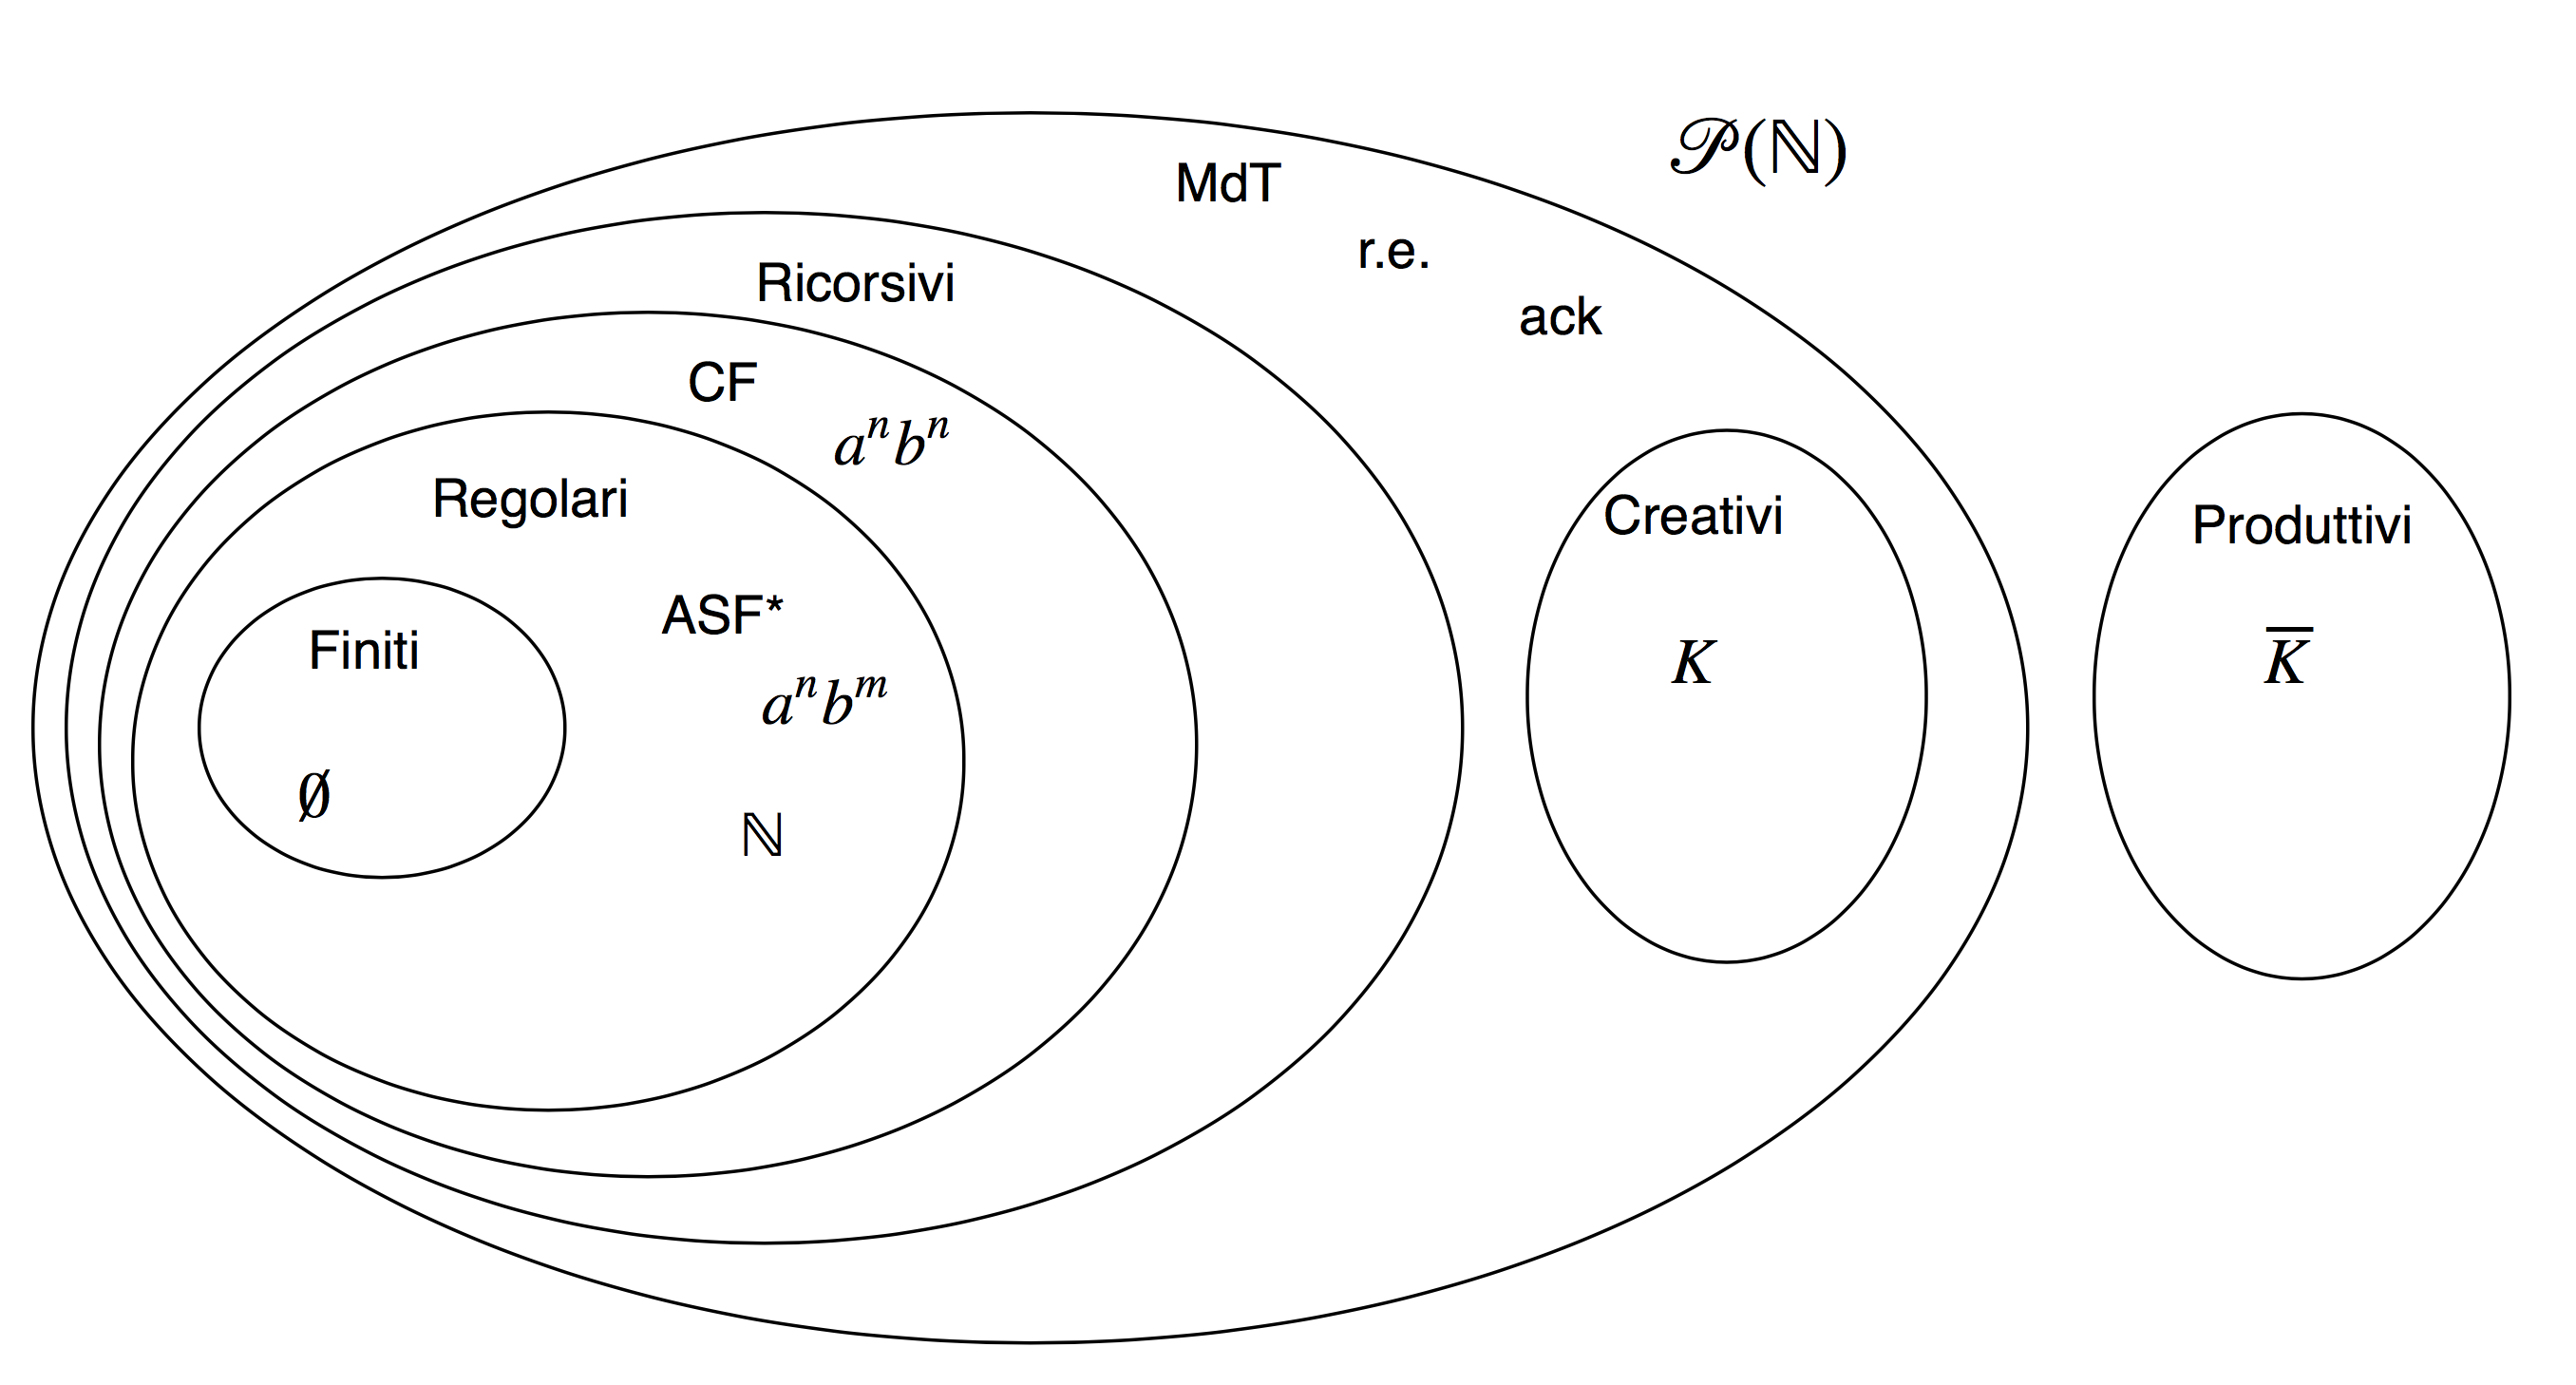
\includegraphics[width=\textwidth]{gerarchia-chomsky}
\end{document}